\documentclass[semifinal]{cpecmu}

%% This is a sample document demonstrating how to use the CPECMU
%% project template. If you are having trouble, see "cpecmu.pdf" for
%% documentation.

\projectNo{P069-1}
\acadyear{2024}

\titleTH{รายงานสหกิจศึกษา}
\titleEN{Cooperative Education Report}

\author{ณัฐพงษ์ เทพพิทักษ์}{Natthaphong Thepphithak}{640610634}
% \author{นายบรรจบ พบเอฟตลอด}{Banjob Pob-eftalord}{690610969}

\cpeadvisor{patiwet}
\cpecommittee{paskorn}
% \committee{รศ.ดร.\,นิพนธ์ ธีรอำพน}{Assoc.\,Prof.\,Nipon Theera-Umpon, Ph.D.}

%% Some possible packages to include:
\usepackage[final]{graphicx} % for including graphics

%% Add bookmarks and hyperlinks in the document.
\PassOptionsToPackage{hyphens}{url}
\usepackage[colorlinks=true,allcolors=Blue4,citecolor=red,linktoc=all]{hyperref}
\def\UrlLeft#1\UrlRight{$#1$}

%% Needed just by this example, but maybe not by most reports
\usepackage{afterpage} % for outputting
\usepackage{pdflscape} % for landscape figures and tables. 
\usepackage{minted}
\usepackage{pdfpages}
\usepackage{hyperref}
\usepackage{pdfpages}
\usepackage{fancyhdr}
\usepackage{import}
\usepackage{longtable}
\usepackage{array}
\usepackage{tabularx}

\fancyhf{}
\fancyfoot[C]{\thepage}

%% Some other useful packages. Look these up to find out how to use
%% them.
% \usepackage{natbib}    % for author-year citation styles
% \usepackage{txfonts}
% \usepackage{appendix}  % for appendices on a per-chapter basis
% \usepackage{xtab}      % for tables that go over multiple pages
% \usepackage{subfigure} % for subfigures within a figure
% \usepackage{pstricks,pdftricks} % for access to special PostScript and PDF commands
% \usepackage{nomencl}   % if you have a list of abbreviations

%% if you're having problems with overfull boxes, you may need to increase
%% the tolerance to 9999
% \tolerance=9999

% \bibliographystyle{plain}
% \bibliographystyle{IEEEbib}
\bibliographystyle{IEEEtran}

% \renewcommand{\topfraction}{0.85}
% \renewcommand{\textfraction}{0.1}
% \renewcommand{\floatpagefraction}{0.75}

%% Example for glossary entry
%% Need to use glossary option
%% See glossaries package for complete documentation.
\ifglossary
  \newglossaryentry{lorem ipsum}{
    name=lorem ipsum,
    description={derived from Latin dolorem ipsum, translated as ``pain itself''}
  }
\fi

%% Uncomment this command to preview only specified LaTeX file(s)
%% imported with \include command below.
%% Any other file imported via \include but not specified here will not
%% be previewed.
%% Useful if your report is large, as you might not want to build
%% the entire file when editing a certain part of your report.
% \includeonly{chapters/intro,chapters/background}

\begin{document}
\maketitle
\makesignature

\ifproject
\begin{abstractTH}
% เขียนบทคัดย่อของรายงานที่นี่

% การเขียนรายงานเป็นส่วนหนึ่งของการทำรายงานวิศวกรรมคอมพิวเตอร์
% เพื่อทบทวนทฤษฎีที่เกี่ยวข้อง อธิบายขั้นตอนวิธีแก้ปัญหาเชิงวิศวกรรม และวิเคราะห์และสรุปผลการทดลองอุปกรณ์และระบบต่างๆ
% \enskip อย่างไรก็ดี การสร้างรูปเล่มรายงานให้ถูกรูปแบบนั้นเป็นขั้นตอนที่ยุ่งยาก
% แม้ว่าจะมีต้นแบบสำหรับใช้ในโปรแกรม Microsoft Word แล้วก็ตาม
% แต่นักศึกษาส่วนใหญ่ยังคงค้นพบว่าการใช้งานมีความซับซ้อน และเกิดความผิดพลาดในการจัดรูปแบบ กำหนดเลขหัวข้อ และสร้างสารบัญอยู่
% \enskip ภาควิชาวิศวกรรมคอมพิวเตอร์จึงได้จัดทำต้นแบบรูปเล่มรายงานโดยใช้ระบบจัดเตรียมเอกสาร
% \LaTeX{} เพื่อช่วยให้นักศึกษาเขียนรายงานได้อย่างสะดวกและรวดเร็วมากยิ่งขึ้น
รายงานนี้เป็นนำเสนอการสหกิจของวิศวกรรมศาสตรสาขาคอมพิวเตอร์ในตำแหน่ง DevOps Engineer 
ที่ SCB TechX ซึ่งเป็นส่วนหนึ่งของธนาคารไทยพาณิชย์ (SCB) 
ในระหว่างช่วงเวลาของการทำงาน ได้มีส่วนร่วมในการสนับสนุนทีมพัฒนาซอฟต์แวร์ โดยเฉพาะในด้านการสร้างและการลบทรัพยากร 
รวมถึงการพัฒนาและบำรุงรักษา Terraform Modules สำหรับโมดูลกลางที่ถูกใช้งานทั้งใน SCB TechX และ SCB ซึ่งทั้งหมดนี้เป็นส่วนสำคัญในการเพิ่มประสิทธิภาพและความคล่องตัวให้กับกระบวนการ DevOps ของ
บริษัท เพื่อตอบสนองความต้องการของลูกค้าอย่างมีประสิทธิภาพและรวดเร็ว
\end{abstractTH}

\begin{abstract}
This report presents a cooperative education experience in Computer Engineering for the position of DevOps Engineer at SCB TechX, a subsidiary of Siam Commercial Bank (SCB). 
During the work period, I participated in supporting the software development team, particularly in the creation and deletion of resources, as well as the development and maintenance of Terraform Modules for central modules used in both SCB TechX and SCB. 
All of these activities were crucial in enhancing the efficiency and agility of the company's DevOps processes to effectively and rapidly meet customer needs.
\end{abstract}

\iffalse
\begin{dedication}
This document is dedicated to all Chiang Mai University students.

Dedication page is optional.
\end{dedication}
\fi % \iffalse

\begin{acknowledgments}
    การที่ข้าพเจ้าได้มาปฏิบัติงานสหกิจศึกษา ณ บริษัท เอสซีบี เทคเอกซ์ จำกัด  ตั้งแต่วันที่ 4 มิถุนายน 2567  ถึง วันที่  25 ตุลาคม 2567  ส่งผลให้ข้าพเจ้าได้รับความรู้และประสบการณ์ต่างๆ ที่มีค่ามากมาย สำหรับรายงานวิชาสหกิจศึกษาฉบับนี้  สำเร็จลงได้ด้วยดีจากความร่วมมือและสนับสนุนจากหลายฝ่าย  ดังนี้
    \begin{enumerate}
        \item พีรวัตร อยู่ใจเย็น ตำแหน่ง Sernior DevOps Engineer
        \item ภัทรพล หมวกมณี ตำแหน่ง DevOps Engineer
    \end{enumerate}
    และบุคคลท่านอื่นๆที่ไม่ได้กล่าวนามทุกท่านที่ได้ให้คำแนะนำช่วยเหลือในการจัดทำรายงาน
	ข้าพเจ้าใคร่ขอขอบพระคุณผู้ที่มีส่วนเกี่ยวข้องทุกท่าน ที่มีส่วนร่วมในการให้ข้อมูล เป็นที่ปรึกษาในการทำรายงานฉบับนี้จนเสร็จสมบูรณ์ ตลอดจนให้การดูแลและให้ความเข้าใจเกี่ยวกับชีวิตของการทำงานจริง ข้าพเจ้าขอขอบคุณ ไว้ ณ ที่นี้
    \acksign{2024}{10}{25}
\end{acknowledgments}%
\fi % \ifproject

\contentspage % generate the table of contents

\ifproject
\tablelistpage
\figurelistpage

% \tablelistpage
\fi % \ifproject

% \abbrlist % this page is optional

% \symlist % this page is optional

% \preface % this section is optional


\pagestyle{empty}\cleardoublepage
\normalspacing \setcounter{page}{1} \pagenumbering{arabic} \pagestyle{cpecmu}

\chapter{\ifenglish Introduction\else ข้อมูลทั่วไปของบรษัท\fi}

\section{\ifenglish Company History\else ประวัติความเป็นมาของบริษัท\fi}

SCB TechX \cite{techxWebsite} ก่อตั้งขึ้นจากความร่วมมือระหว่าง SCBX กลุ่มธุรกิจการเงินและเทคโนโลยีชั้นนำของไทย และ Publicis Sapient บริษัทที่ปรึกษาด้านดิจิทัลทรานส์ฟอร์เมชันระดับโลก มีจุดมุ่งหมายเพื่อมอบบริการด้านเทคโนโลยีที่ตอบสนองความต้องการของธุรกิจต่าง ๆ ตั้งแต่การสร้างนวัตกรรมและผลิตภัณฑ์ใหม่ ไปจนถึงการนำเทคโนโลยีมาเพิ่มประสิทธิภาพในการดำเนินงาน

บริษัทมีความเชี่ยวชาญในการพัฒนาโซลูชันในระดับองค์กร (Enterprise-grade solutions) ที่ปลอดภัยและรองรับการใช้งานของฐานลูกค้าจำนวนมาก นอกจากนี้ SCB TechX ยังจัดองค์กรในรูปแบบ Startup เพื่อลดความซ้ำซ้อนในการทำงานและส่งเสริมความคิดริเริ่มใหม่ ๆ ทำให้สามารถพัฒนาโซลูชันให้กับลูกค้าได้อย่างรวดเร็วและมีประสิทธิภาพ


\section{\ifenglish Company Product\else บริการและผลิตภัณฑ์ของบริษัท\fi}
SCB TechX นำเสนอนวัตกรรมที่พร้อมใช้งานหลากหลายด้าน \cite{techxProduct} ทั้งระบบยืนยันตัวตนแบบดิจิทัลด้วยระบบ KYC \cite{whatIsKYC} ซึ่งทางบริษัทจะเรียกว่า eKYC และแพลตฟอร์มทางการเงินที่หลากหลาย นวัตกรรมเหล่านี้สามารถเชื่อมต่อกับระบบของลูกค้าได้อย่างรวดเร็วและง่ายดาย พร้อมทั้งปรับแต่งตามความต้องการเฉพาะของธุรกิจ ส่งผลให้ลูกค้าของ SCB TechX สามารถเปิดตัวบริการใหม่หรือยกระดับการให้บริการได้อย่างทันท่วงที

นอกจากนี้ SCB TechX ยังให้บริการที่ครอบคลุมด้านการให้คำปรึกษาทางเทคโนโลยี (Technology Consulting), โซลูชันด้านโครงสร้างพื้นฐานและแพลตฟอร์ม (Infrastructure \& Platforms), โซลูชันคลาวด์ (Cloud Solutions), แพลตฟอร์มเทคโนโลยีแบบครบวงจร (xPlatform), การจัดการข้อมูลและความปลอดภัย (Data \& Security), และโซลูชันด้านข้อมูลและ AI (TechX Data \& AI Solutions) ที่ออกแบบมาเพื่อรองรับและเสริมสร้างศักยภาพให้กับธุรกิจในยุคดิจิทัล

\clearpage

\section{\ifenglish Organization\else ผู้บริหารของบริษัท\fi}
\begin{figure}[ht]
    \begin{center}
    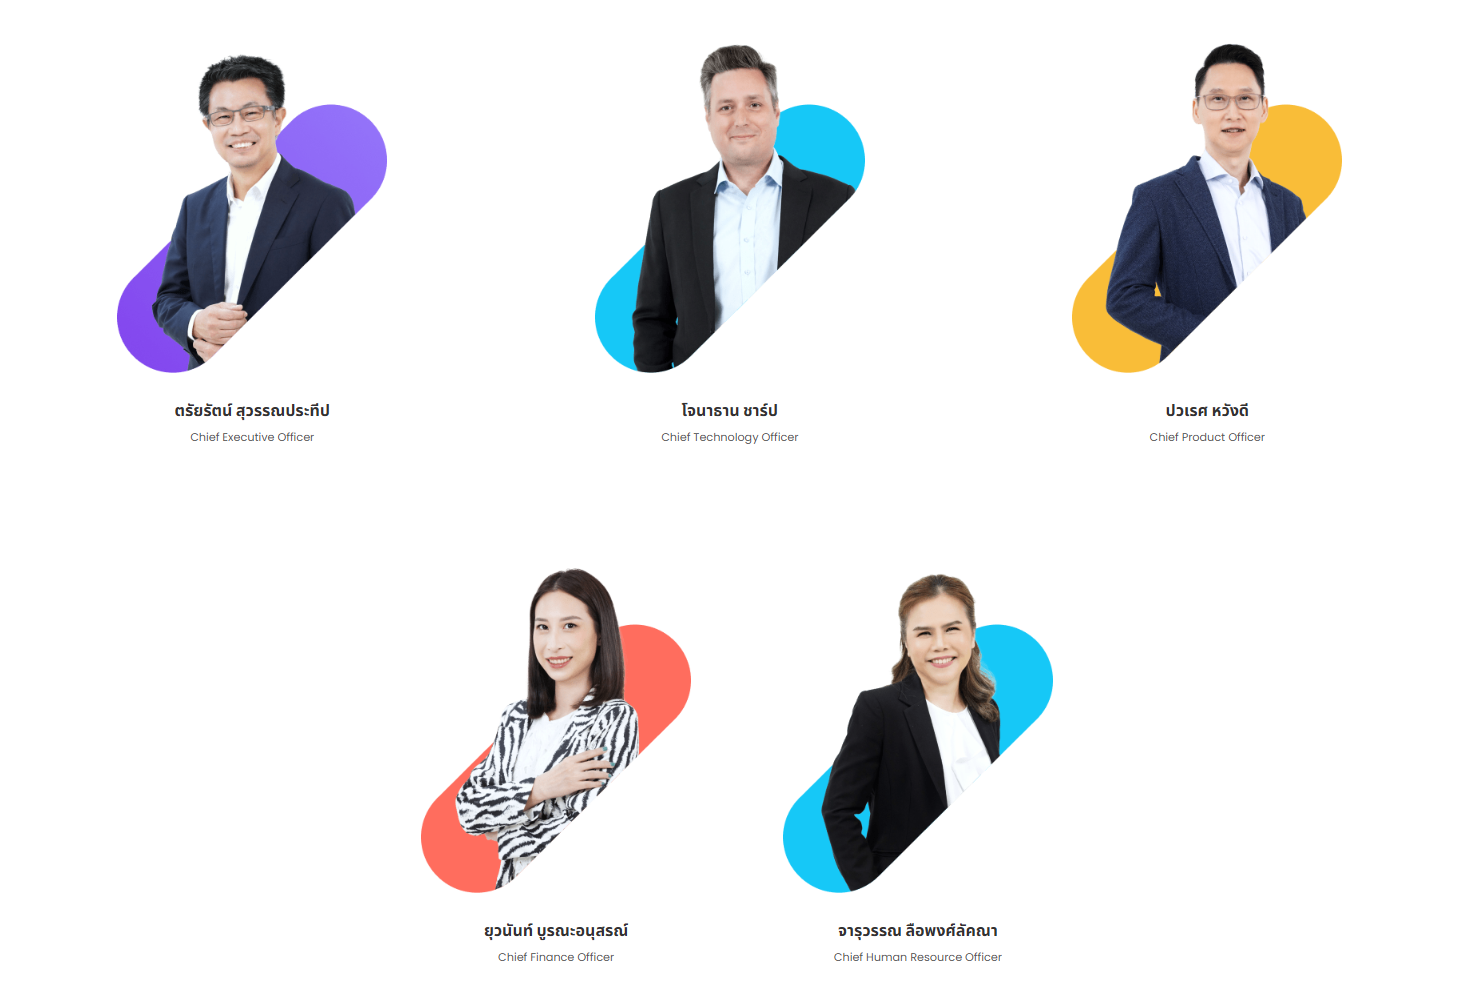
\includegraphics[scale=0.3]{images/org.png}
    \end{center}
    \caption[Board Of Director]{ผู้บริหารและตำแหน่งของบริษัท}
    \label{fig:org}
\end{figure}

% \section{\ifenglish Objectives\else วัตถุประสงค์ของโครงงาน\fi}
% \begin{enumerate}
%     \item
% \end{enumerate}

% \section{\ifenglish Project scope\else ขอบเขตของโครงงาน\fi}

% \subsection{\ifenglish Hardware scope\else ขอบเขตด้านฮาร์ดแวร์\fi}

% \subsection{\ifenglish Software scope\else ขอบเขตด้านซอฟต์แวร์\fi}

% \section{\ifenglish Expected outcomes\else ประโยชน์ที่ได้รับ\fi}

% \section{\ifenglish Technology and tools\else เทคโนโลยีและเครื่องมือที่ใช้\fi}

% \subsection{\ifenglish Hardware technology\else เทคโนโลยีด้านฮาร์ดแวร์\fi}

% \subsection{\ifenglish Software technology\else เทคโนโลยีด้านซอฟต์แวร์\fi}

% \section{\ifenglish Project plan\else แผนการดำเนินงาน\fi}

% \begin{plan}{6}{2020}{2}{2021}
%     \planitem{7}{2020}{8}{2020}{ศึกษาค้นคว้า}
%     \planitem{8}{2020}{1}{2021}{ชิล}
%     \planitem{2}{2021}{2}{2021}{เผา}
%     \planitem{12}{2019}{1}{2022}{ทดสอบ}
% \end{plan}

% \section{\ifenglish Roles and responsibilities\else บทบาทและความรับผิดชอบ\fi}
% อธิบายว่าในการทำงาน นศ. มีการกำหนดบทบาทและแบ่งหน้าที่งานอย่างไรในการทำงาน จำเป็นต้องใช้ความรู้ใดในการทำงานบ้าง

% \section{\ifenglish%
% Impacts of this project on society, health, safety, legal, and cultural issues
% \else%
% ผลกระทบด้านสังคม สุขภาพ ความปลอดภัย กฎหมาย และวัฒนธรรม
% \fi}

% แนวทางและโยชน์ในการประยุกต์ใช้งานโครงงานกับงานในด้านอื่นๆ รวมถึงผลกระทบในด้านสังคมและสิ่งแวดล้อมจากการใช้ความรู้ทางวิศวกรรมที่ได้

% Define groups of JIRA cards
\newcommand{\supportJiraCards}{
  XDO-7387 & CBS-SunCBS | Destroy Dev02 resources \\
  XDO-7389 & CBS-SunCBS Request to add role to managed identity \\
  XDO-7394 & CBS-MCR | Provisioning Storage Account for Dev01 and QA01 \\
  XDO-7421 & CBS-SunCBS | Request to set parameter on MySQL to Off on IaC \\
  *XDO-7422 & CBS-DAP | Setup ADF to send diagnostic log to DAP log analytic workspace \\
  XDO-7429 & Require provision the existing azure manage identity to version v.1.2.1 \\
  *XDO-7444 & CBS-SunCBS Request to install teleport for MySQL flexible servers \\
  XDO-7453 & CBS MCR | Request to grant db\_datareader access to the Azure Automation Account user-managed identity \\
  XDO-7490 & CBS-SunCBS | setup Mysql parameter on QA01 \\
  XDO-7604 & CBS-SunCBS | Provisioning Infrastructure resource for Migration-Dev1 (DEV03) \\
  XDO-7686 & CBS-SunCBS | Asssement of changing Storage account ADLS Gen2 \\
  XDO-7745 & CBS-SunCBS | Change storage account from General to ADLS Gen2 on Dev01 \\
}

\newcommand{\developJiraCards}{
  XDO-7423 & POC ADF Storage Event Trigger Over SFTP
  XDO-7483 & [ADF][linked-services] Convert module from IAC next gen to xplatform multicloud \\
  XDO-7484 & [ADF][trigger] Convert module from IAC next gen to xplatform multicloud \\
  XDO-7561 & CBS-DAP | Enhance Azure Data factory linked services modules \\
  XDO-7633 & [PYMD] Develop check appconfig for Azure Databrick \\
  XDO-7737 & [CBS] Update linked service catalog to support custom sftp \\
  XDO-7742 & [CBS] Create Linked Services documentation \\
  XDO-7743 & CBS-SunCBS | Research on Entra ID with CosmosDB for PostgreSQL \\
  XDO-7744 & [CBS] | POC Dynamic create trigger via ARM Template\\
  XDO-7760 & [CBS] Make the ADF dynamic trigger document \\
}

% Create a table of JIRA cards with hyperlinks
\newcommand{\jiradata}{
  \begin{center}
    \begin{tabular}{|c|p{0.7\textwidth}|}
      \hline
      \multicolumn{1}{|c|}{\textbf{รหัส Jira Card}} & \multicolumn{1}{c|}{\textbf{หัวข้องาน}} \\
      \hline
      \multicolumn{2}{|c|}{\textbf{Support Cards}}                                         \\
      \hline
      \supportJiraCards
      \hline
      \multicolumn{2}{|c|}{\textbf{Develop Cards}}                                         \\
      \hline
      \developJiraCards
      \hline
    \end{tabular}
  \end{center}
}

% Helper command to create hyperlinks
\newcommand{\jiralink}[1]{\hyperref[desc:#1]{\texttt{#1}}}

\setcounter{secnumdepth}{3}

\chapter{\ifenglish Cooperative Details\else รายเอียดการไปสหกิจศึกษา\fi}


\section{\ifenglish Foundation of DevOps\else ปรับความรู้พื้นฐานของการเป็น DevOps\fi}
แนวทางในการเริ่มต้นทำงานในสายงาน DevOps จำเป็นต้องมีการศึกษาและปรับพื้นฐานความรู้ที่สำคัญเพื่อให้แน่ใจว่าพร้อมสำหรับการทำงานจริง
เนื่องจาก DevOps เป็นสายงานที่มีความใหม่และมีการพัฒนาอย่างต่อเนื่องในวงการซอฟต์แวร์ โดยหัวข้อที่ได้รับมอบหมายให้ศึกษาเพื่อเตรียมความพร้อมจะประกอบด้วย

\begin{itemize}
      \item \textbf{Docker}: เครื่องมือสำหรับการทำ Containerization เพื่อเพิ่มประสิทธิภาพในการพัฒนาและการส่งมอบซอฟต์แวร์
      \item \textbf{Kubernetes}: ระบบสำหรับการทำ Orchestration และจัดการคอนเทนเนอร์ที่ทำงานในสเกลใหญ่
      \item \textbf{Jenkins}: เครื่องมือสำหรับการทำ Continuous Integration/Continuous Deployment (CI/CD) เพื่อเพิ่มความรวดเร็วและลดข้อผิดพลาดในการพัฒนาซอฟต์แวร์
      \item \textbf{Terraform \& IaC}: เครื่องมือสำหรับการทำ Infrastructure as Code (IaC) เพื่อจัดการและปรับแต่งโครงสร้างพื้นฐานด้วยโค้ด
      \item \textbf{Monitoring Tools}: เครื่องมือที่ใช้ในการตรวจสอบและติดตามการทำงานของระบบอย่างมีประสิทธิภาพ
      \item \textbf{ELK Stack}: ระบบสำหรับการจัดการและวิเคราะห์ข้อมูล Logging เพื่อช่วยในการตรวจสอบและวิเคราะห์ปัญหาในระบบ
\end{itemize}

ทั้งนี้การศึกษาหัวข้อเหล่านี้มีระยะเวลาประมาณ 2-4 สัปดาห์ และท้ายสุดจะต้องมีการนำเสนอสิ่งที่ได้เรียนรู้
ให้กับพี่ ๆ ในทีมได้ฟังและประเมิณว่าพร้อมที่จะทำงานจริงหรือไม่ อย่างไรก็ตามรายละเอียดในหัวข้อย่อยต่าง ๆ หลังจากนี้จะเป็นการนำเสนอสิ่งที่ได้เรียนรู้และได้นำมาประยุกต์ใช้ในการทำงานจริง
ส่วนหัวข้อนอกเหนือจากที่จะกล่าวถึงก็สำคัญไม่น้อยเช่นกันแต่จะข้อนำเสนอ Documentation ที่ได้ทำสรุปการเรียนรู้มาแล้วนั้นในส่วนภาคผนวก

% \import{chapters/detail_sections}{docker.tex}
% \clearpage
% \import{chapters/detail_sections}{kube.tex}
\clearpage
\import{chapters/detail_sections}{jenkins.tex}
\clearpage
\import{chapters/detail_sections}{terraform.tex}
\clearpage

\section{\ifenglish TOR\else TOR\fi}เนื่องจากการมาสหกิจศึกษาจำเป็นต้องมีการประเมิณที่เข้มงวด ดังนั้นจึงได้จัดทำ TOR ขึ้นเพื่อเป็นมาตรฐานในการทำงานและประเมิณผลงานมราควรจะทำได้ดังนี้
\begin{itemize}
      \item ทำงานในลักษณะของ Task based จำนวณ 30 tasks เป็นขึ้นต่ำ เนื่องจากทีม DevOps ของ SCB Techx ไม่ได้ใช้การทำงานแบบ Agile จึงทำให้ลักษณะการจะเป็น Kanban กล่าวคือ เมื่อมีงานใหม่เข้ามาจะสามารถทำได้ทันทีโดยไม่ต้องมีการ Sprint planning ก่อน ดังนั้นเองการทำงานจึงต้องอาศัยความรอบคอบและความรวดเร็วในการทำงาน เพื่อตอบสนองความต้องการของทีม Dev และ ลูกค้าให้ได้มากที่สุด
\end{itemize}
ดังนั้นรายหัวข้อต่อไปจะเป็นการนำเสนอ Task งานที่ได้รับมอบหมายให้ทำทั้งหมด เพื่อแสดงให้เห็นว่าสามารถบรรลุเป้าหมายของ TOR ได้

\section{\ifenglish Responsibity Task\else งานที่ได้รับมอบหมาย\fi}
สืบเนื่องจากงานที่ได้รับมอบหมายนั้นจะเป็นในลักษณะ Task งาน ดังนั้นใน Section นี้จะนำเสนอ Task งานที่ได้ทั้งหมดพร้อมทั้งรายละเอียดของแต่ละ Task งานที่ได้รับมอบหมาย โดยจะแบ่งออกได้เป็น 2 กลุ่มใหญ่ ๆ คือ Task งานที่เป็น Support และ Task งานที่เป็น Develop
\subsection{\ifenglish Support Task\else งาน Support\fi}
\begin{itemize}
      \item \textbf{XDO-7387:} CBS-SunCBS | Destroy Dev02 resources \\
            งานนี้จะต้อง Destroy Resource ที่อยู่ใน Dev02 ของ Sun-CBS Project เนื่องจากเกิดข้อผิดพลาดในการวางแผนการใช้งาน Resource ทำให้สิ้นเปลือง Cost โดยไม่จำเป็น
      \item \textbf{XDO-7389:} CBS-SunCBS Request to add role to managed identity \\
            งานนี้สืบเนื่องมาจาก Dev Request ให้ DevOps เพิ่ม Role ในการ login เข้าใช้งานให้กับ Managed Identity เนื่องจาก Managed Identity ไม่มีสิทธิการใช้งานในส่วนที่ Dev ต้องการจึงต้องทำการเพิ่มให้ภายหลัง
      \item \textbf{XDO-7394:} CBS-MCR | Provisioning Storage Account for Dev01 and QA01 \\
            งานนี้จะต้องทำการ Provision Storage Account ให้กับ Dev01 และ QA01 ของ MCR Project ตาม Planing ที่ได้กำหนดไว้
      \item \textbf{XDO-7421 | XDO-7490:} CBS-SunCBS | Request to set parameter on MySQL to Off on IaC\\
            งานนี้จะต้องหาวิธีการในการปิด Parameter บางอย่างใน MySQL ซึ่งมีข้อจำจัดคือจะต้องทำผ่าน Terraform เท่านั้น
      \item \textbf{XDO-7429:} Require provision the existing azure manage identity to version v.1.2.1\\
            งานนี้เป็นงานที่ทีม Platfrom ได้เปิดการ์ดแบบด่วนเข้ามาทีม DevOps เพิ่มให้อัพเดท Module Terraform สำหรับการสร้าง Azure Manage Identity เป็น version 1.2.1 (ล่าสุด ณ ขณะนั้น) เพื่อให้สอดคล้องกับ Pipeline ใหม่ของ Platform Team ที่จะถูกนำมาใช้งาน
      \item \textbf{XDO-7453:} CBS MCR | Request to grant db\_datareader access to the Azure Automation Account user-managed identity\\
            งานนี้เป็นการเพิ่ม Role ให้กับ Azure Automation Account ที่ใช้งานใน MCR Project เพื่อให้สามารถอ่านข้อมูลจาก Database ได้ ซึ่ง Role นั้นก็อาศัยการใช้ Managed Identity ในการ Login นั้นหมายความว่า Managed Identity อันนี้จะต้องผ่านการเพิ่ม Login Role มาแล้วคล้ายๆกับงาน XDO-7389
      \item \textbf{XDO-7604:} CBS-SunCBS | Provisioning Infrastructure resource for Migration-Dev1 (DEV03)\\
            งานที่เป็นการ Provision Infrastructure ให้กับ Environment ใหม่ที่ชื่อว่า Dev03 ซึ่งหมายความว่า Resource ทุกอย่างไม่เคยมีมาก่อนและต้องทำการสร้างขึ้นมาใหม่ทั้งหมดประกอบไปด้วย
            \begin{itemize}
                  \item Storage Account
                  \item Managed Identity
                  \item Redis Cache
                  \item Mysql flexible server
                  \item CosmosDB
                  \item Key vault
            \end{itemize}
            ซึ่ง Spec ของแต่ละรายการจะถูกกำหนดไว้ใน Jira Card นั้น ๆ และการสร้าง Resource ทุกอย่างนี้จะต้องผ่านการใช้ Terraform และมจะีลำดับการสร้างเพื่อไม่ให้เกิด COnflict ในการสร้าง Resource ดังนั้นเองงานนี้จึงต้องมีความเข้าใจและรอบคอบในการทำงาน
      \item \textbf{XDO-7686 | XDO-7745:} CBS-SunCBS | Asssement of changing Storage account ADLS Gen2\\
            งานนี้คือการเปลี่ยน Version ของ Storage Account จาก General ไปเป็น ADLS Gen2 ซึ่งเป็นการเปลี่ยนแปลงที่สำคัญเพื่อเพิ่มประสิทธิภาพในการใช้งานของ Storage Account โดยเฉพาะในการใช้งานในส่วนของ Data Lake ซึ่งการเปลี่ยนแปลง Version นั้นจะต้องเกิดการลบและสร้างขึ้นมาใหม่ทั้งหมดดังนั้นก่อนเริ่มดำเนินการจะต้องมีการ Approve จาก Dev ต้นทางซึ่งเป็นเจ้าของข้อมูลที่อยู่ใน Storage Account นั้น และงานลักษณะนี้จะต้องทำในหลายๆ Environment เช่นกัน
\end{itemize}

\subsection{\ifenglish Develop Task\else งาน Develop\fi}
\begin{itemize}
      \item \textbf{XDO-7483 | XDO-7484:} [ADF] Convert module from IAC next gen to xplatform multicloud\\
            งานเป็นงานที่คล้ายๆการ Restructure IaC ของการสร้าง ADF ในโปรเจค Payment Domain ใหม่ทั้งหมดเนื่องจาก Version ปัจจุบันนั้นไม่ได้แยก Module ของแต่ละ Component ของ ADF ออกจากกันซึ่งประกอบด้วย Datafactory, Linked services, Trigger และ Pipeline ส่งผลให้เมื่อมีความต้องการในแก้ไขบางอย่างจะต้องพบเจอกับ Code ประมาณ 10,000 บรรทัด ซึ่งเป็นเรื่องที่ไม่ควรจะเกิดขึ้น ทางทีม DevOps จึงเห็นว่าเรื่องนี้ควรจะแก้ไข ซึ่งงานนี้ผมได้ทำกับพี่เลี้ยงอีกคนหนึ่ง โดยผมรับหน้าที่ในการ Restructure ส่วนของ Linked Services และ Trigger ซึ่งเป็นส่วนที่มีความซับซ้อนมากที่สุด โดยการ Restructure ครั้งนี้อ้างอิง Standard ของ Module จากฝั่ง SCB ที่ทาง DevOps ของ Techx เป็นผู้ Design ขึ้นมา ทั้งหมดใช้เวลาประมาณ 2 สัปดาห์ในการ Implement และ Test
      \item \textbf{XDO-7561 | XDO-7737 | XDO-7742:} CBS-DAP | Enhance Azure Data factory linked services modules
            งานนี้เป็นการเพิ่มความสร้างมาของ SFTP Linked Services ใน ADF Modole ของ SCB ให้สามารถไปดึงรหัสผ่านของ SFTP server จาก Azure keyvault ได้ โดยที่ไม่ต้องใส่รหัสผ่านลงใน Config ของ ADF โดยตรง ซึ่งเป็นเรื่องที่สำคัญในการเพิ่มความปลอดภัยในการใช้งานของ ADF และเป็นการเพิ่มความสะดวกในการใช้งานด้วย

            หลังจาก Enhance ฝั่ง Module หลักไปแล้วก็ต้องไปแก้ไข Catalog ที่เรียกใช้ Module ให้รองรับการใช้งาน Feature นี้ได้เช่นกันโดย Catalog จะเป็นฝั่ง Techx ที่รับหน้าที่ดูแลให้

            ทั้งนี้การที่เรา Develop Module เช่นเพิ่ม Feature ใหม่เข้ามาจะต้องมีการทำ Documentation ของวิธีการใช้ Module นั้นขึ้นมางานนี้ก็เช่นกันผมต้องทำ Documentation เพื่อสอนการใช้งาน SFTP Linked Services ที่ผมได้พัฒนาขึ้นมา ซึ่ง Document จะต้องเป็นภาษาอังกฤษ เนื่องจากมีทีมพัฒนาที่เป็นต่างชาติอยู่ใน Project นี้ด้วย
      \item \textbf{XDO-7633:} [PYMD] Develop check appconfig for Azure Databrick
            งานนี้เเป็น Request จาก Dev ที่มีปัญหาก่อนการ Deploy Production ว่าต้องการ Jenkins Pipeline ซักตัวหนึ่งที่ใช้ในการ Check Config ของ Microservcice ใน Release นั้น ๆ ที่กำลังจะ Deploy ว่าได้มีการ Config ถูกต้องหรือไม่ โดยที่ Config ที่ต้องการ Check นั้นจะเป็น Config ที่เกี่ยวข้องกับ Azure Databrick ซึ่งเป็น Service ที่ใช้ในการทำงานกับ Big Data ซึ่ง Config file นั้นมีอยู๋หลากหลายรูปแบบไม่ว่าจะเป็น YAML, JSON ซึ่งนั้นก็เป็นความถ้าทายของผมที่จะต้องทำให้ Check ได้ทุกรูปแบบไฟล์ โดยที่ Logic การเช็คจะเขียนด้วย Python และจะต้องทำงานผ่าน Jenkins ดังนั้นก็จะต้องมีการเขียน Jenkins Pipelien ขึ้นมาด้วยนั้นเอง
\end{itemize}

\subsection{\ifenglish POC\else งาน Prove Of Concept\fi}
\begin{itemize}
      \item \textbf{XDO-7423:} POC ADF Storage Event Trigger Over SFTP\\
            งานนี้ทางทีม Dev ได้ถามาทางทีม DevOps มาว่า Trigger ชนิด Blob Event trigger ใน ADF นั้นสามารถ trigger เมื่อมี File อัพโหลดผ่าน SFTP เข้าไปได้หรือไม่ ซึงผมเองได้รับหน้าที่ในการหาคำตอบเรื่องนี้จีงได้ตอบมาว่า สามารถทำงานได้แต่ไม่ใช่ Solution ที่ทาง Microsoft ให้มา แต่จะเป็นการ Custom Header Parameter บางตัวเข้าไปใน Trigger เพื่อทำให้ Trigger เองสามารถตัวจับ Event ที่มาจาก SFTP ได้
      \item \textbf{XDO-7743:} CBS-SunCBS | Research on Entra ID with CosmosDB for PostgreSQL
      \item \textbf{XDO-7744 | XDO-7760:} [CBS] | POC Dynamic create trigger via ARM Template and Documentation
\end{itemize}

\section{\ifenglish Benefit\else สวัสดิการที่ได้รับ\fi}
บริษัท SCB TechX ให้ความสำคัญกับเรื่องของสวัสดิการที่ดีให้กับพนักงาน โดยเฉพาะนักศึกษาสหกิจศึกษาที่เข้ามาทำงานในบริษัท
ถึงแม้จะไม่ได้เป็นพนักงานประจำ แต่ก็ได้รับสวัสดิการที่ดีจากบริษัทอย่างเช่น
\begin{itemize}
      \item MacBook Pro ให้ใช้งานตลอดระยะทำงาน ซึ่งจะเป็นเครื่องประจำของคนนั้นๆเลย
      \item อาหารเช้าและน้ำดื่มฟรีทุกวันทำงาน
      \item Account ของแหล่งเรียนรู้ออนไลน์เช่น Udemy ที่สามารถเรียน Course ไหน ๆ ก็ได้ฟรี
      \item กิจกรรมพัฒนานักศึกษาฝึกงานและสหกิจศึกษาทั้งด้าน Soft Skill และ Hard Skill ตลอดระยะเวลาทำงาน
      \item เบี้ยเลี้ยงในการทำงาน 500 บาท / วันทำงาน (ไม่นับวันมี่ลา หรือวันหยุด)
\end{itemize}
ทั้งนี้ทั้งหมดหมดที่กล่าวมาเป็นเพียงส่วนหนึ่งของสวัสดิการที่ได้รับจากบริษัท SCB TechX และยังมีสวัสดิการอื่น ๆ ที่ยังไม่ได้กล่าวถึง

\chapter{\ifenglish Conclusion\else สรุปผลการปฏิบัติงาน\fi}

\section{สรุปผลการศึกษา/การฝึกปฏิบัติงาน} ตามข้อตกลงในเอกสารเงื่อนไขการประเมินผลการปฏิบัติงาน (TOR) ซึ่งได้กำหนดให้ต้องดำเนินงานให้แล้วเสร็จไม่น้อยกว่า 30 งาน ในช่วงระยะเวลาของการฝึกปฏิบัติงาน ข้าพเจ้าได้ดำเนินการแล้วเสร็จจำนวน 32 งาน ทั้งนี้ รายละเอียดของแต่ละงานได้ถูกสรุปไว้ในส่วนของรายงานก่อนหน้านี้อย่างครบถ้วน

จากการดำเนินงานที่กล่าวมาข้างต้น ข้าพเจ้าสามารถบรรลุเป้าหมายของการฝึกปฏิบัติงานตามที่ได้กำหนดไว้ ซึ่งถือเป็นการบรรลุผลสำเร็จตามเกณฑ์ที่วางไว้

\section{ประโยชน์ที่ได้รับจากการศึกษา/การฝึกปฏิบัติงาน}
การฝึกปฏิบัติสหกิจศึกษาที่บริษัท SCB TechX ในตำแหน่ง \textit{Trainee DevOps Engineer} ตลอดระยะเวลา 5 เดือนนั้น ทำให้ผมได้รับประสบการณ์ที่มีค่ามากมาย โดยเฉพาะการทำงานร่วมกับทีมและการเรียนรู้ทักษะใหม่ ๆ ที่ไม่เคยได้ศึกษามาก่อน การได้รับโอกาสจากพี่ ๆ ในทีมและหัวหน้างานที่คอยช่วยเหลือและให้คำแนะนำเป็นสิ่งสำคัญมาก โดยเฉพาะพี่เลี้ยงของผมที่ให้ความไว้วางใจและเปิดโอกาสให้ผมได้ลองผิดลองถูกในการทำงานจริง ซึ่งช่วยพัฒนาทักษะและความมั่นใจในการทำงานอย่างมาก ทำให้ประสบการณ์สหกิจศึกษาครั้งนี้ประสบความสำเร็จ

ในส่วนของ \textit{Hard Skills} ที่ได้เรียนรู้ หนึ่งในสิ่งที่สำคัญคือการได้ลองใช้งาน \textit{Azure Cloud Provider} ซึ่งเป็นความรู้ที่ไม่ได้เรียนในห้องเรียน การได้เห็นและทดลองใช้ \textit{Azure} กับระบบจริงของธนาคาร ซึ่งเป็นระบบที่มีความซับซ้อนและสำคัญมาก ทำให้ผมเข้าใจถึงการออกแบบและการจัดการระบบที่ซับซ้อนมากขึ้น พี่เลี้ยงของผมได้มอบหมายงานเกี่ยวกับ \textit{Azure} ให้ผมรับผิดชอบส่วนใหญ่ ทำให้ผมได้เรียนรู้วิธีการใช้งาน \textit{Azure} อย่างลึกซึ้ง และได้นำความรู้นี้ไปปรับใช้ใน \textit{โปรเจคจบ} ของผม ทั้งในด้านการออกแบบสถาปัตยกรรมระบบ (\textit{System Architecture}) และการประยุกต์ใช้ \textit{Azure} ให้เหมาะสมกับโปรเจค

นอกจากนี้ \textit{Soft Skills} ก็เป็นสิ่งที่ผมได้พัฒนาระหว่างการทำงานในสหกิจครั้งนี้ บริษัท SCB TechX มีกิจกรรมให้เข้าร่วมเป็นประจำเพื่อส่งเสริม \textit{Soft Skills} เช่น การทำงานร่วมกับคนต่าง \textit{Generation}, ทักษะการสื่อสาร, การเข้าสังคม และการสร้างโปรไฟล์สำหรับการสมัครงานในอนาคต กิจกรรมเหล่านี้ช่วยให้ผมพัฒนาความสามารถในการทำงานร่วมกับผู้อื่นและสร้างเครือข่ายที่ดีสำหรับอนาคต

\section{ข้อเสนอจากบริษัท}
จากการพูดคุยอย่างไม่เป็นทางการกับหัวหน้างาน ทราบว่าทางทีม DevOps ของบริษัท SCB TechX ไม่มีตำแหน่งว่างในขณะนี้ จึงไม่มีข้อเสนอรับเข้าทำงานในตำแหน่งนี้ อย่างไรก็ตาม หัวหน้าทีม DevOps Manager (Platform Service Manager) ได้แนะนำให้สมัครในตำแหน่งอื่นที่ไม่ใช่ DevOps โดยแนะนำตำแหน่ง Platform Engineer ซึ่งมีลักษณะงานที่ไม่แตกต่างจาก DevOps มากนัก ทั้งนี้ในระหว่างการฝึกงาน ผมมีโอกาสได้ช่วยงานทีม Platform Engineer อยู่บ้าง จึงเชื่อว่าสามารถทำงานในตำแหน่งนี้ได้โดยไม่ต้องมีการสอนงานเพิ่มเติมมากนัก นอกจากนี้ ยังมีโอกาสเปลี่ยนแปลงตำแหน่งภายหลังได้ตามความเหมาะสม

ในส่วนของฐานเงินเดือนเริ่มต้นของบริษัทนั้นอยู่ที่ 30,000 บาทต่อเดือน โดยอาจปรับเพิ่มได้ตามประสบการณ์และความสามารถของผู้สมัคร

% \chapter{\ifenglish Background Knowledge and Theory\else ทฤษฎีที่เกี่ยวข้อง\fi}

การทำโครงงาน เริ่มต้นด้วยการศึกษาค้นคว้า ทฤษฎีที่เกี่ยวข้อง หรือ งานวิจัย/โครงงาน ที่เคยมีผู้นำเสนอไว้แล้ว ซึ่งเนื้อหาในบทนี้ก็จะเกี่ยวกับการอธิบายถึงสิ่งที่เกี่ยวข้องกับโครงงาน เพื่อให้ผู้อ่านเข้าใจเนื้อหาในบทถัด ๆ ไปได้ง่ายขึ้น

\section{The first section}
The text for Section 1 goes here.

\section{Second section}
Section 2 text.

\subsection{Subsection heading goes here}

Subsection 1 text

\subsubsection{Subsubsection 1 heading goes here}
Subsubsection 1 text

\subsubsection{Subsubsection 2 heading goes here}
Subsubsection 2 text

\section{Third section}
Section 3 text. The dielectric constant\index{dielectric constant}
at the air-metal interface determines
the resonance shift\index{resonance shift} as absorption or capture occurs
is shown in Equation~\eqref{eq:dielectric}:

\begin{equation}\label{eq:dielectric}
k_1=\frac{\omega}{c({1/\varepsilon_m + 1/\varepsilon_i})^{1/2}}=k_2=\frac{\omega
\sin(\theta)\varepsilon_\mathit{air}^{1/2}}{c}
\end{equation}

\noindent
where $\omega$ is the frequency of the plasmon, $c$ is the speed of
light, $\varepsilon_m$ is the dielectric constant of the metal,
$\varepsilon_i$ is the dielectric constant of neighboring insulator,
and $\varepsilon_\mathit{air}$ is the dielectric constant of air.

\section{About using figures in your report}

% define a command that produces some filler text, the lorem ipsum.
\newcommand{\loremipsum}{
  \textit{Lorem ipsum dolor sit amet, consectetur adipisicing elit, sed do
  eiusmod tempor incididunt ut labore et dolore magna aliqua. Ut enim ad
  minim veniam, quis nostrud exercitation ullamco laboris nisi ut
  aliquip ex ea commodo consequat. Duis aute irure dolor in
  reprehenderit in voluptate velit esse cillum dolore eu fugiat nulla
  pariatur. Excepteur sint occaecat cupidatat non proident, sunt in
  culpa qui officia deserunt mollit anim id est laborum.}\par}

\begin{figure}
  \centering

  \fbox{
     \parbox{.6\textwidth}{\loremipsum}
  }

  % To include an image in the figure, say myimage.pdf, you could use
  % the following code. Look up the documentation for the package
  % graphicx for more information.
  % \includegraphics[width=\textwidth]{myimage}

  \caption[Sample figure]{This figure is a sample containing \gls{lorem ipsum},
  showing you how you can include figures and glossary in your report.
  You can specify a shorter caption that will appear in the List of Figures.}
  \label{fig:sample-figure}
\end{figure}

Using \verb.\label. and \verb.\ref. commands allows us to refer to
figures easily. If we can refer to Figures
\ref{fig:walrus} and \ref{fig:sample-figure} by name in the {\LaTeX}
source code, then we will not need to update the code that refers to it
even if the placement or ordering of the figures changes.

\loremipsum\loremipsum

% This code demonstrates how to get a landscape table or figure. It
% uses the package lscape to turn everything but the page number into
% landscape orientation. Everything should be included within an
% \afterpage{ .... } to avoid causing a page break too early.
\afterpage{
  \begin{landscape}
  \begin{table}
    \caption{Sample landscape table}
    \label{tab:sample-table}

    \centering

    \begin{tabular}{c||c|c}
        Year & A & B \\
        \hline\hline
        1989 & 12 & 23 \\
        1990 & 4 & 9 \\
        1991 & 3 & 6 \\
    \end{tabular}
  \end{table}
  \end{landscape}
}

\loremipsum\loremipsum\loremipsum

\section{Overfull hbox}

When the \verb.semifinal. option is passed to the \verb.cpecmu. document class,
any line that is longer than the line width, i.e., an overfull hbox, will be
highlighted with a black solid rule:
\begin{center}
\begin{minipage}{2em}
juxtaposition
\end{minipage}
\end{center}

\section{\ifenglish%
\ifcpe CPE \else ISNE \fi knowledge used, applied, or integrated in this project
\else%
ความรู้ตามหลักสูตรซึ่งถูกนำมาใช้หรือบูรณาการในโครงงาน
\fi
}

อธิบายถึงความรู้ และแนวทางการนำความรู้ต่าง ๆ ที่ได้เรียนตามหลักสูตร ซึ่งถูกนำมาใช้ในโครงงาน

\section{\ifenglish%
Extracurricular knowledge used, applied, or integrated in this project
\else%
ความรู้นอกหลักสูตรซึ่งถูกนำมาใช้หรือบูรณาการในโครงงาน
\fi
}

อธิบายถึงความรู้ต่าง ๆ ที่เรียนรู้ด้วยตนเอง และแนวทางการนำความรู้เหล่านั้นมาใช้ในโครงงาน

% \chapter{\ifproject%
\ifenglish Project Structure and Methodology\else โครงสร้างและขั้นตอนการทำงาน\fi
\else%
\ifenglish Project Structure\else โครงสร้างของรายงาน\fi
\fi
}

ในบทนี้จะกล่าวถึงหลักการ และการออกแบบระบบ

\makeatletter

% \renewcommand\section{\@startsection {section}{1}{\z@}%
%                                    {13.5ex \@plus -1ex \@minus -.2ex}%
%                                    {2.3ex \@plus.2ex}%
%                                    {\normalfont\large\bfseries}}

\makeatother
%\vspace{2ex}
% \titleformat{\section}{\normalfont\bfseries}{\thesection}{1em}{}
% \titlespacing*{\section}{0pt}{10ex}{0pt}

\section{Alice in Wonderland}

\begin{figure}
\begin{center}
\includegraphics{800px-Briny_Beach.jpg}
\end{center}
\caption[Poem]{The Walrus and the Carpenter}
\label{fig:walrus}
\end{figure}

\subsection{The Black Kitten}
  One thing was certain, that the WHITE kitten had had nothing to
do with it:---it was the black kitten's fault entirely~\cite{aiw}.  For the
white kitten had been having its face washed by the old cat for
the last quarter of an hour (and bearing it pretty well,
considering); so you see that it COULDN'T have had any hand in
the mischief.

  The way Dinah washed her children's faces was this:  first she
held the poor thing down by its ear with one paw, and then with
the other paw she rubbed its face all over, the wrong way,
beginning at the nose:  and just now, as I said, she was hard at
work on the white kitten, which was lying quite still and trying
to purr---no doubt feeling that it was all meant for its good.

  But the black kitten had been finished with earlier in the
afternoon, and so, while Alice was sitting curled up in a corner
of the great arm-chair, half talking to herself and half asleep,
the kitten had been having a grand game of romps with the ball of
worsted Alice had been trying to wind up, and had been rolling it
up and down till it had all come undone again; and there it was,
spread over the hearth-rug, all knots and tangles, with the
kitten running after its own tail in the middle.

\subsection{The Reproach}

  `Oh, you wicked little thing!' cried Alice, catching up the
kitten, and giving it a little kiss to make it understand that it
was in disgrace.  `Really, Dinah ought to have taught you better
manners!  You OUGHT, Dinah, you know you ought!' she added,
looking reproachfully at the old cat, and speaking in as cross a
voice as she could manage---and then she scrambled back into the
arm-chair, taking the kitten and the worsted with her, and began
winding up the ball again.  But she didn't get on very fast, as
she was talking all the time, sometimes to the kitten, and
sometimes to herself.  Kitty sat very demurely on her knee,
pretending to watch the progress of the winding, and now and then
putting out one paw and gently touching the ball, as if it would
be glad to help, if it might.

  `Do you know what to-morrow is, Kitty?' Alice began.  `You'd
have guessed if you'd been up in the window with me---only Dinah
was making you tidy, so you couldn't.  I was watching the boys
getting in stick for the bonfire---and it wants plenty of
sticks, Kitty!  Only it got so cold, and it snowed so, they had
to leave off.  Never mind, Kitty, we'll go and see the bonfire
to-morrow.'  Here Alice wound two or three turns of the worsted
round the kitten's neck, just to see how it would look:  this led
to a scramble, in which the ball rolled down upon the floor, and
yards and yards of it got unwound again.

  `Do you know, I was so angry, Kitty,' Alice went on as soon as
they were comfortably settled again, `when I saw all the mischief
you had been doing, I was very nearly opening the window, and
putting you out into the snow!  And you'd have deserved it, you
little mischievous darling!  What have you got to say for
yourself?  Now don't interrupt me!' she went on, holding up one
finger.  `I'm going to tell you all your faults.  Number one:
you squeaked twice while Dinah was washing your face this
morning.  Now you can't deny it, Kitty:  I heard you!  What that
you say?' (pretending that the kitten was speaking.)  `Her paw
went into your eye?  Well, that's YOUR fault, for keeping your
eyes open---if you'd shut them tight up, it wouldn't have
happened.  Now don't make any more excuses, but listen!  Number
two:  you pulled Snowdrop away by the tail just as I had put down
the saucer of milk before her!  What, you were thirsty, were you?

% \chapter{\ifproject%
\ifenglish Experimentation and Results\else การทดลองและผลลัพธ์\fi
\else%
\ifenglish System Evaluation\else การประเมินระบบ\fi
\fi}

ในบทนี้จะทดสอบเกี่ยวกับการทำงานในฟังก์ชันหลัก ๆ

\ifproject
  % \chapter{\ifenglish Conclusions and Discussions\else บทสรุปและข้อเสนอแนะ\fi}

\section{\ifenglish Conclusions\else สรุปผล\fi}

นศ. ควรสรุปถึงข้อจำกัดของระบบในด้านต่าง ๆ ที่ระบบมีในเนื้อหาส่วนนี้ด้วย

\section{\ifenglish Challenges\else ปัญหาที่พบและแนวทางการแก้ไข\fi}

ในการทำโครงงานนี้ พบว่าเกิดปัญหาหลัก ๆ ดังนี้

\section{\ifenglish%
Suggestions and further improvements
\else%
ข้อเสนอแนะและแนวทางการพัฒนาต่อ
\fi
}

ข้อเสนอแนะเพื่อพัฒนาโครงงานนี้ต่อไป มีดังนี้

\fi

\bibliography{sampleReport}

\ifproject
  \normalspacing
  \appendix
  % \chapter{เอกสารสำคัญที่เกี่ยวข้อง}
\begin{itemize}
    \item \textbf{เอกสารสำคัญของคณะ}
          \begin{itemize}
              \item \hyperlink{target:03-04}{วศ.สก.-03/04 รายงานตัวเข้าสหกิจศึกษา} (หน้า \pageref{page:03-04})
              \item \hyperlink{target:03}{วศ.ฝ.ค-03 แบบฟอร์มยืนยันการรับนักศึกษา} (หน้า \pageref{page:03})
              \item \hyperlink{target:11}{วศ.สก.-11 แบบสรุปผลการปฏิบัติงานสหกิจศึกษา} (หน้า \pageref{page:11})
          \end{itemize}
    \item \textbf{เอกสารสำคัญที่เกี่ยวข้องกับงาน}
          \begin{itemize}
              \item \hyperlink{target:docker}{เอกสารสรุปสิ่งที่ได้เรียนรู้และลองทำ Docker} (หน้า \pageref{page:docker})
              \item \hyperlink{target:kube}{เอกสารสรุปสิ่งที่ได้เรียนรู้และลองทำ Kubernetes} (หน้า \pageref{page:kube})
              \item \hyperlink{target:jenkins}{เอกสารสรุปสิ่งที่ได้เรียนรู้และลองทำ Jenkins} (หน้า \pageref{page:jenkins})
              \item \hyperlink{target:terraform}{เอกสารสรุปสิ่งที่ได้เรียนรู้และลองทำ Terraform} (หน้า \pageref{page:terraform})
              \item \hyperlink{target:monitoring}{เอกสารสรุปสิ่งที่ได้เรียนรู้เกี่ยวกับ Monitoring Tools} (หน้า \pageref{page:monitoring})
              \item \hyperlink{target:elk}{เอกสารสรุปสิ่งที่ได้เรียนรู้เกี่ยวกับ ELK Stack} (หน้า \pageref{page:elk})
          \end{itemize}
\end{itemize}

% คณะ
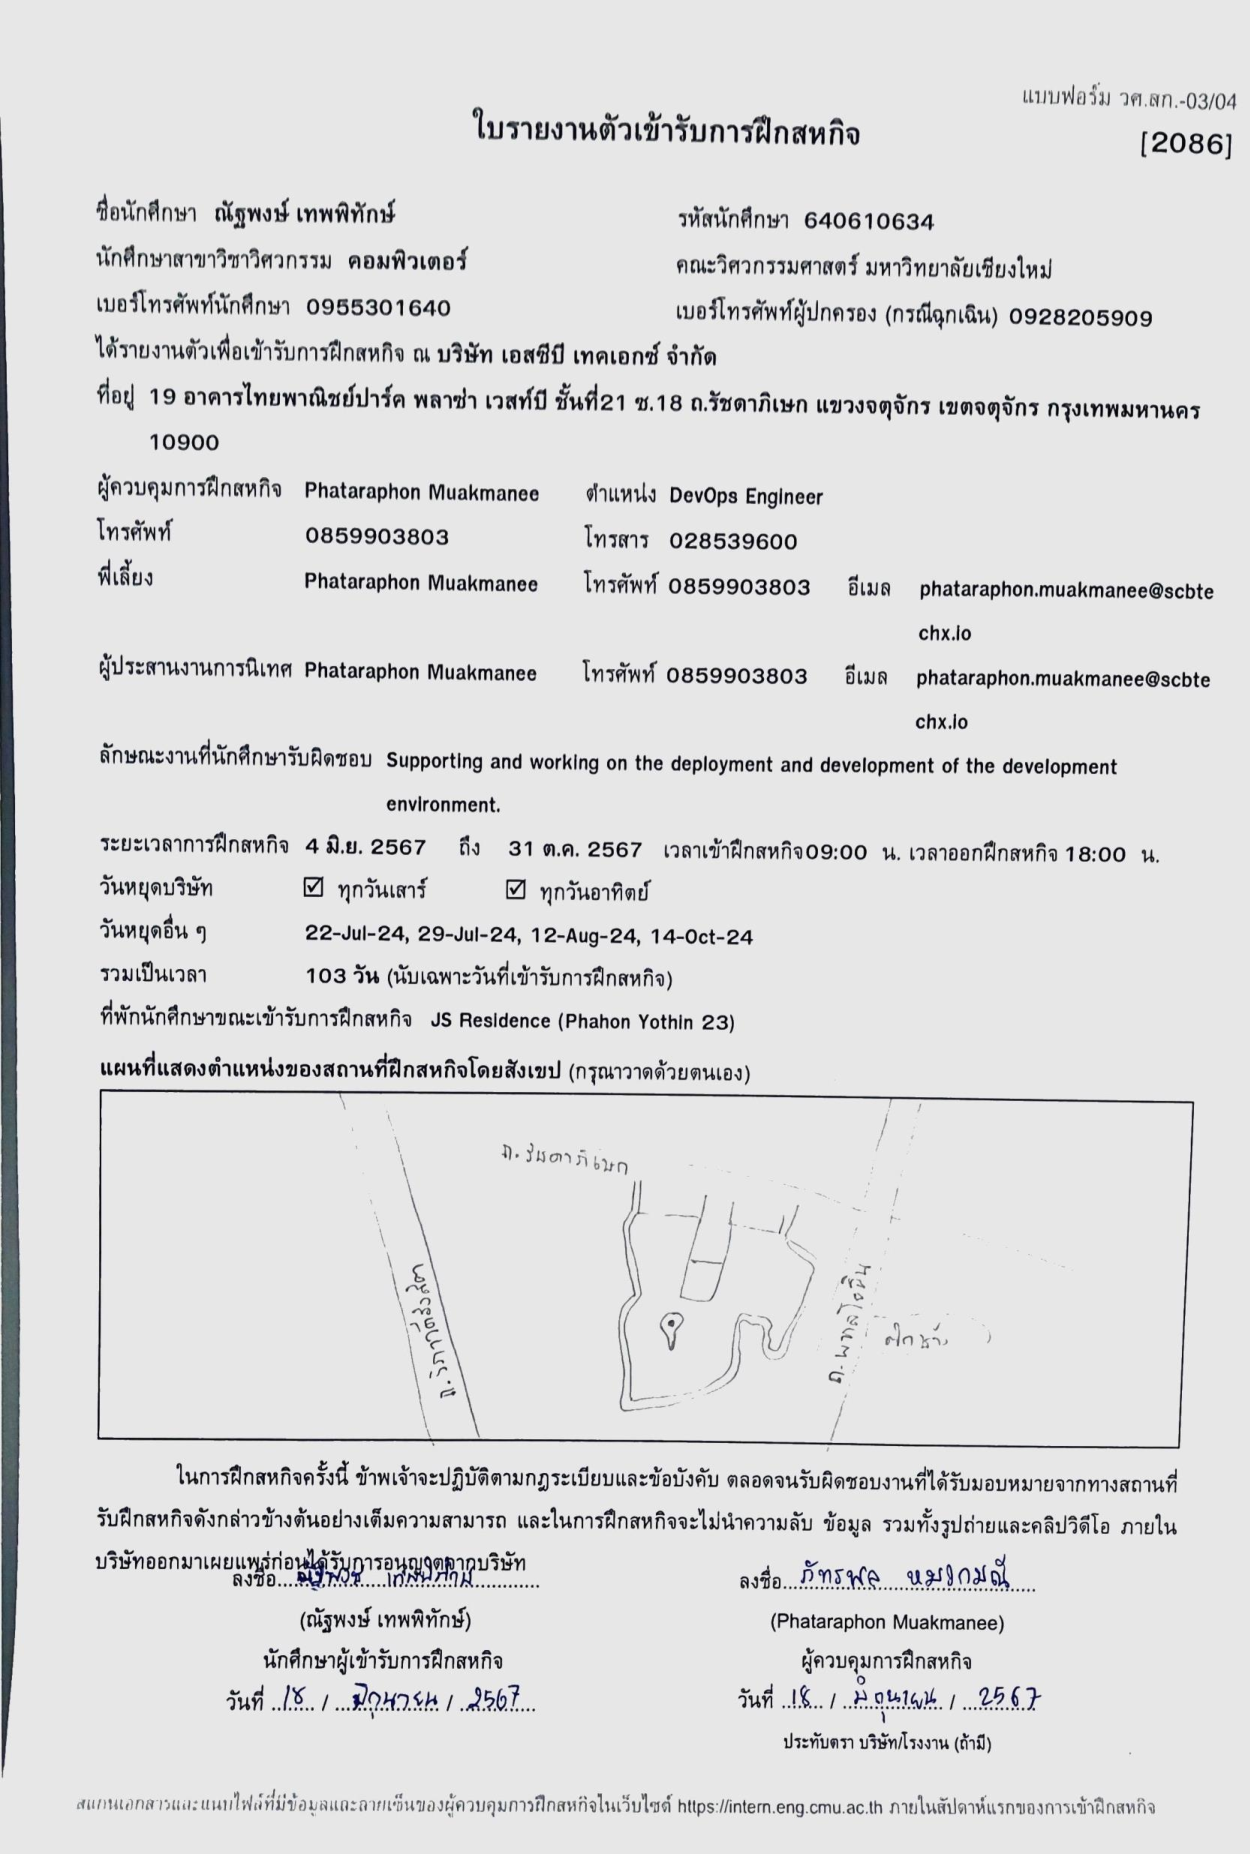
\includepdf[pages=-, scale=.8, pagecommand={\hypertarget{target:03-04}{},\label{page:03-04}}, nup=1x1, frame=true]{pdf/03-04}
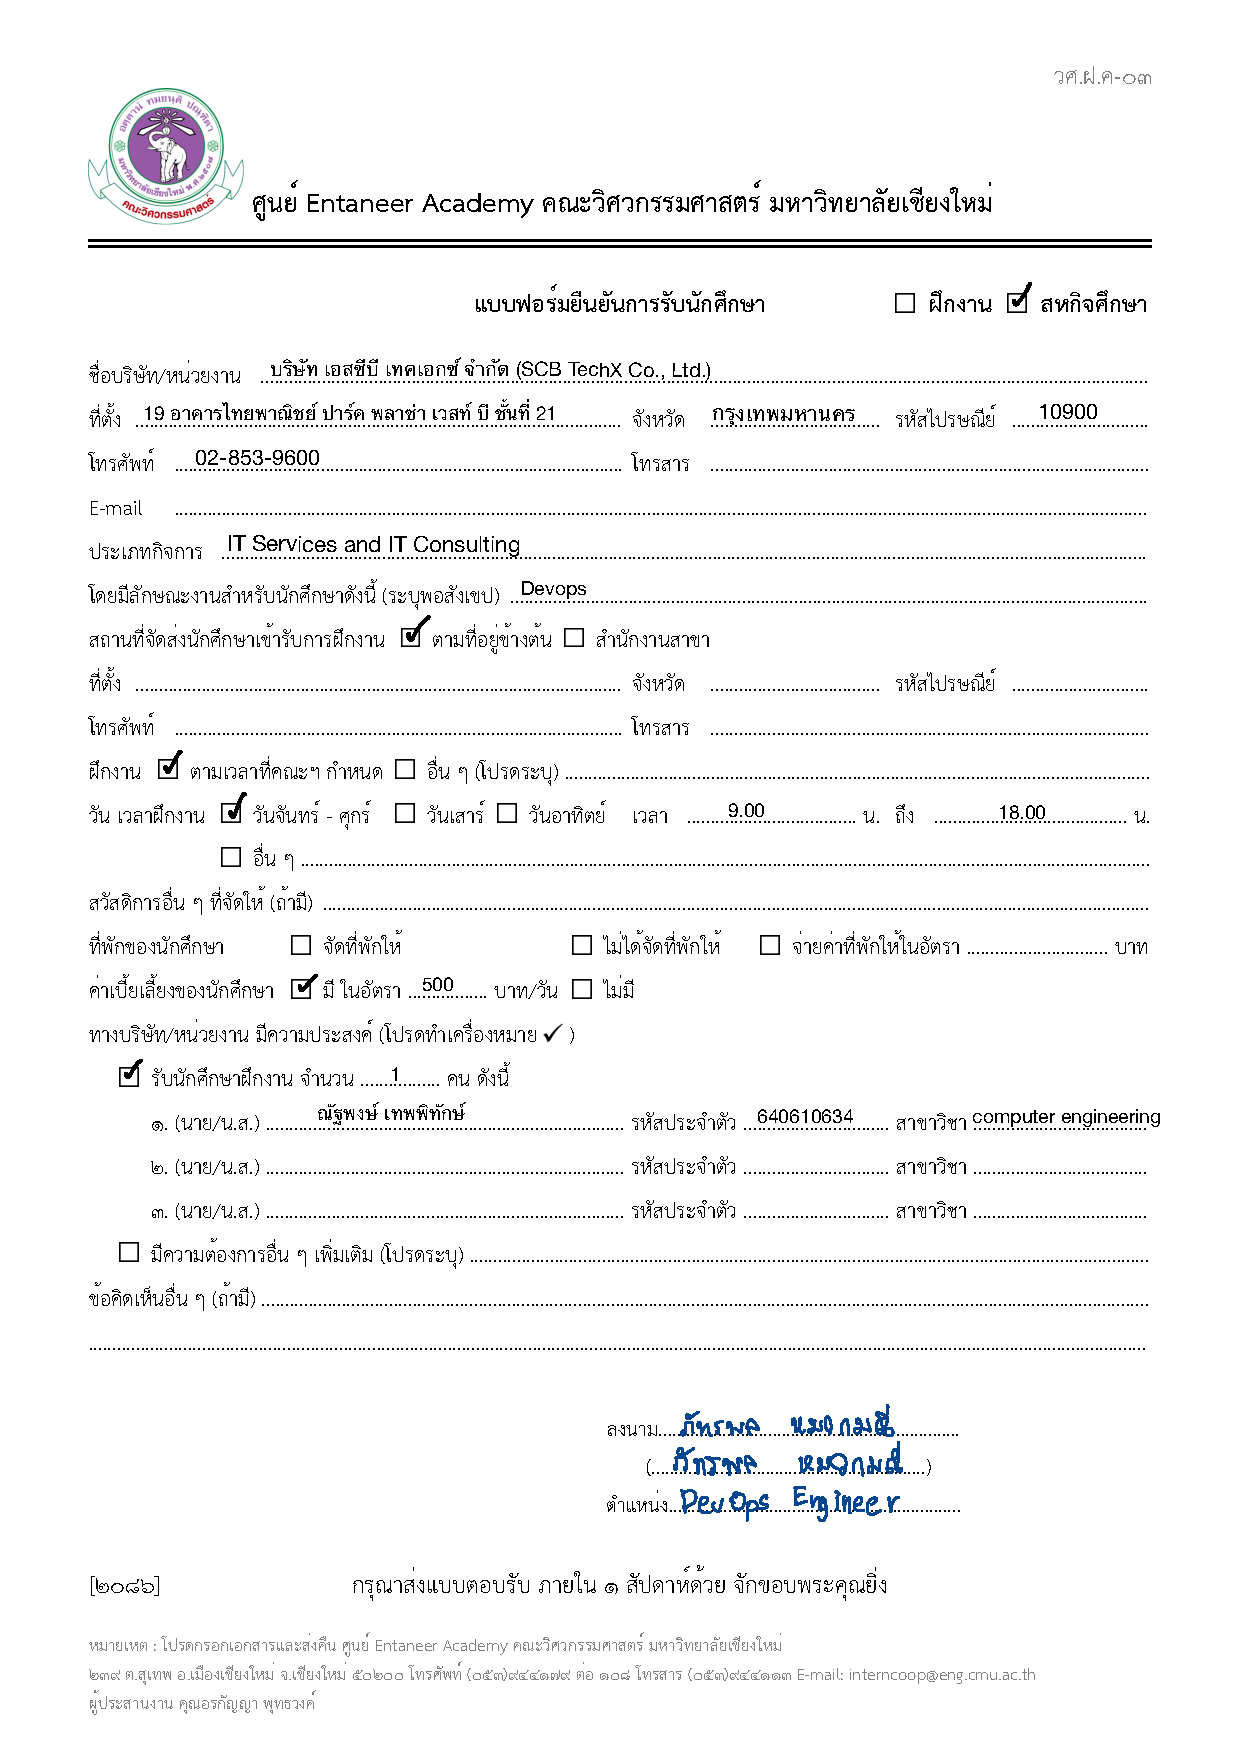
\includepdf[pages=-, scale=.8, pagecommand={\hypertarget{target:03}{},\label{page:03}}, nup=1x1, frame=true]{pdf/03}
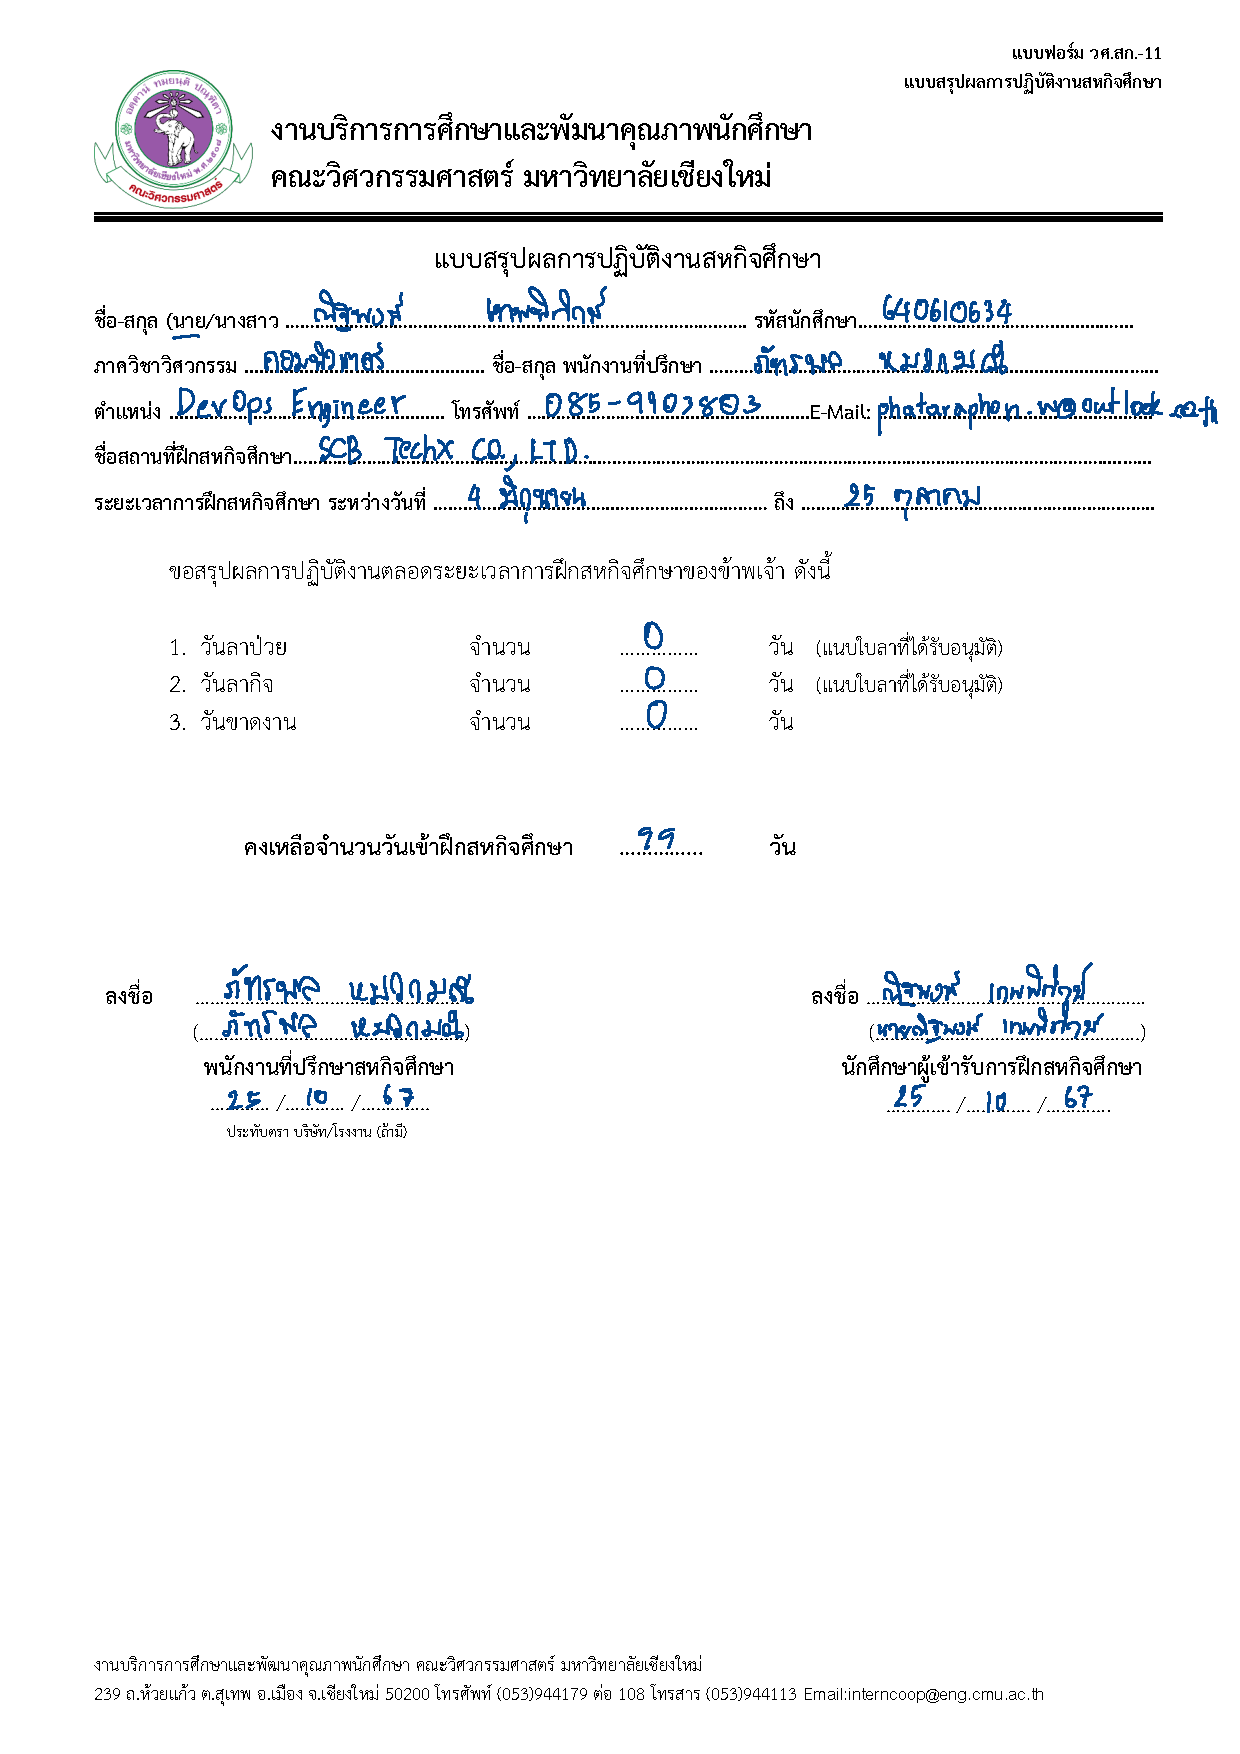
\includepdf[pages=-, scale=.8, pagecommand={\hypertarget{target:11}{},\label{page:11}}, nup=1x1, frame=true]{pdf/11}

% ส่วนที่เกี่ยวข้อง
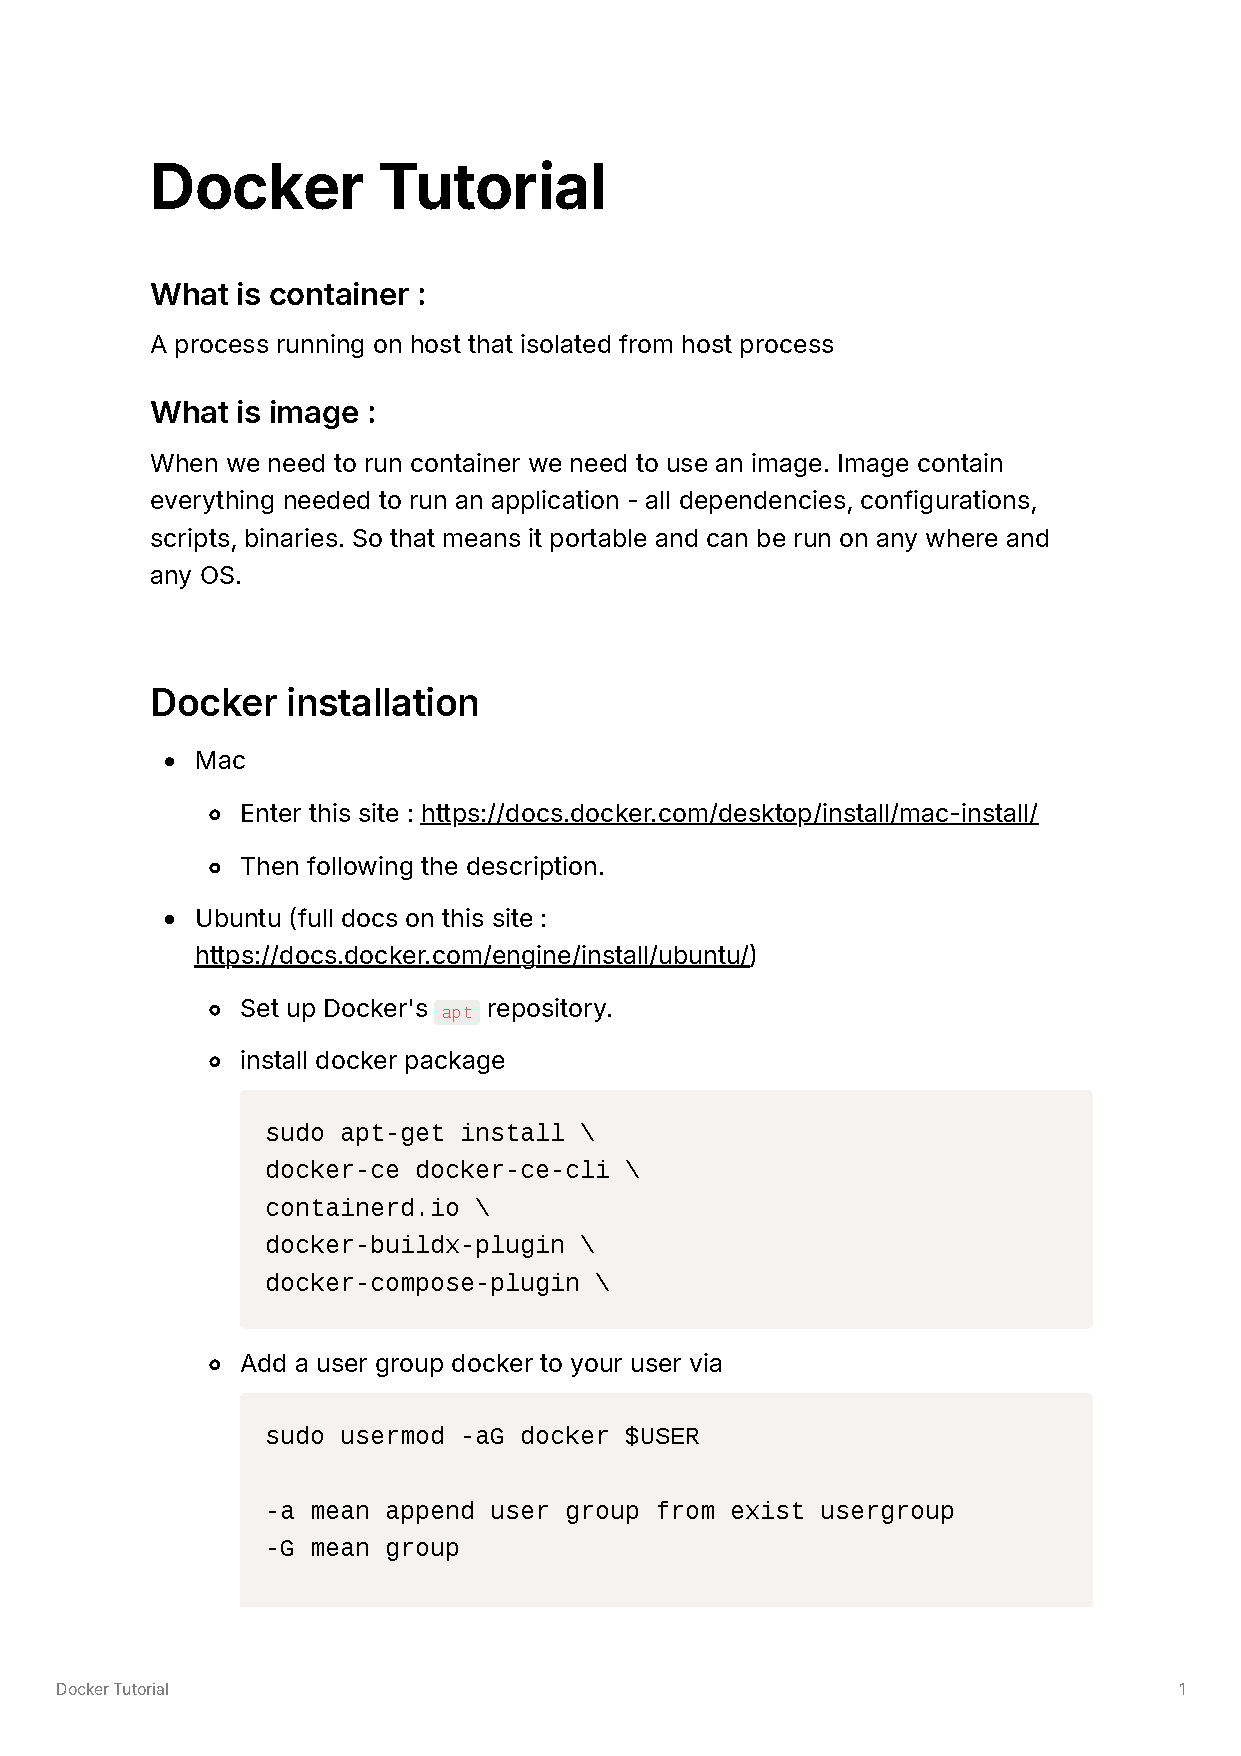
\includepdf[pages=-, scale=.8, pagecommand={\hypertarget{target:docker}{},\label{page:docker}}, nup=1x1, frame=true]{pdf/docker}
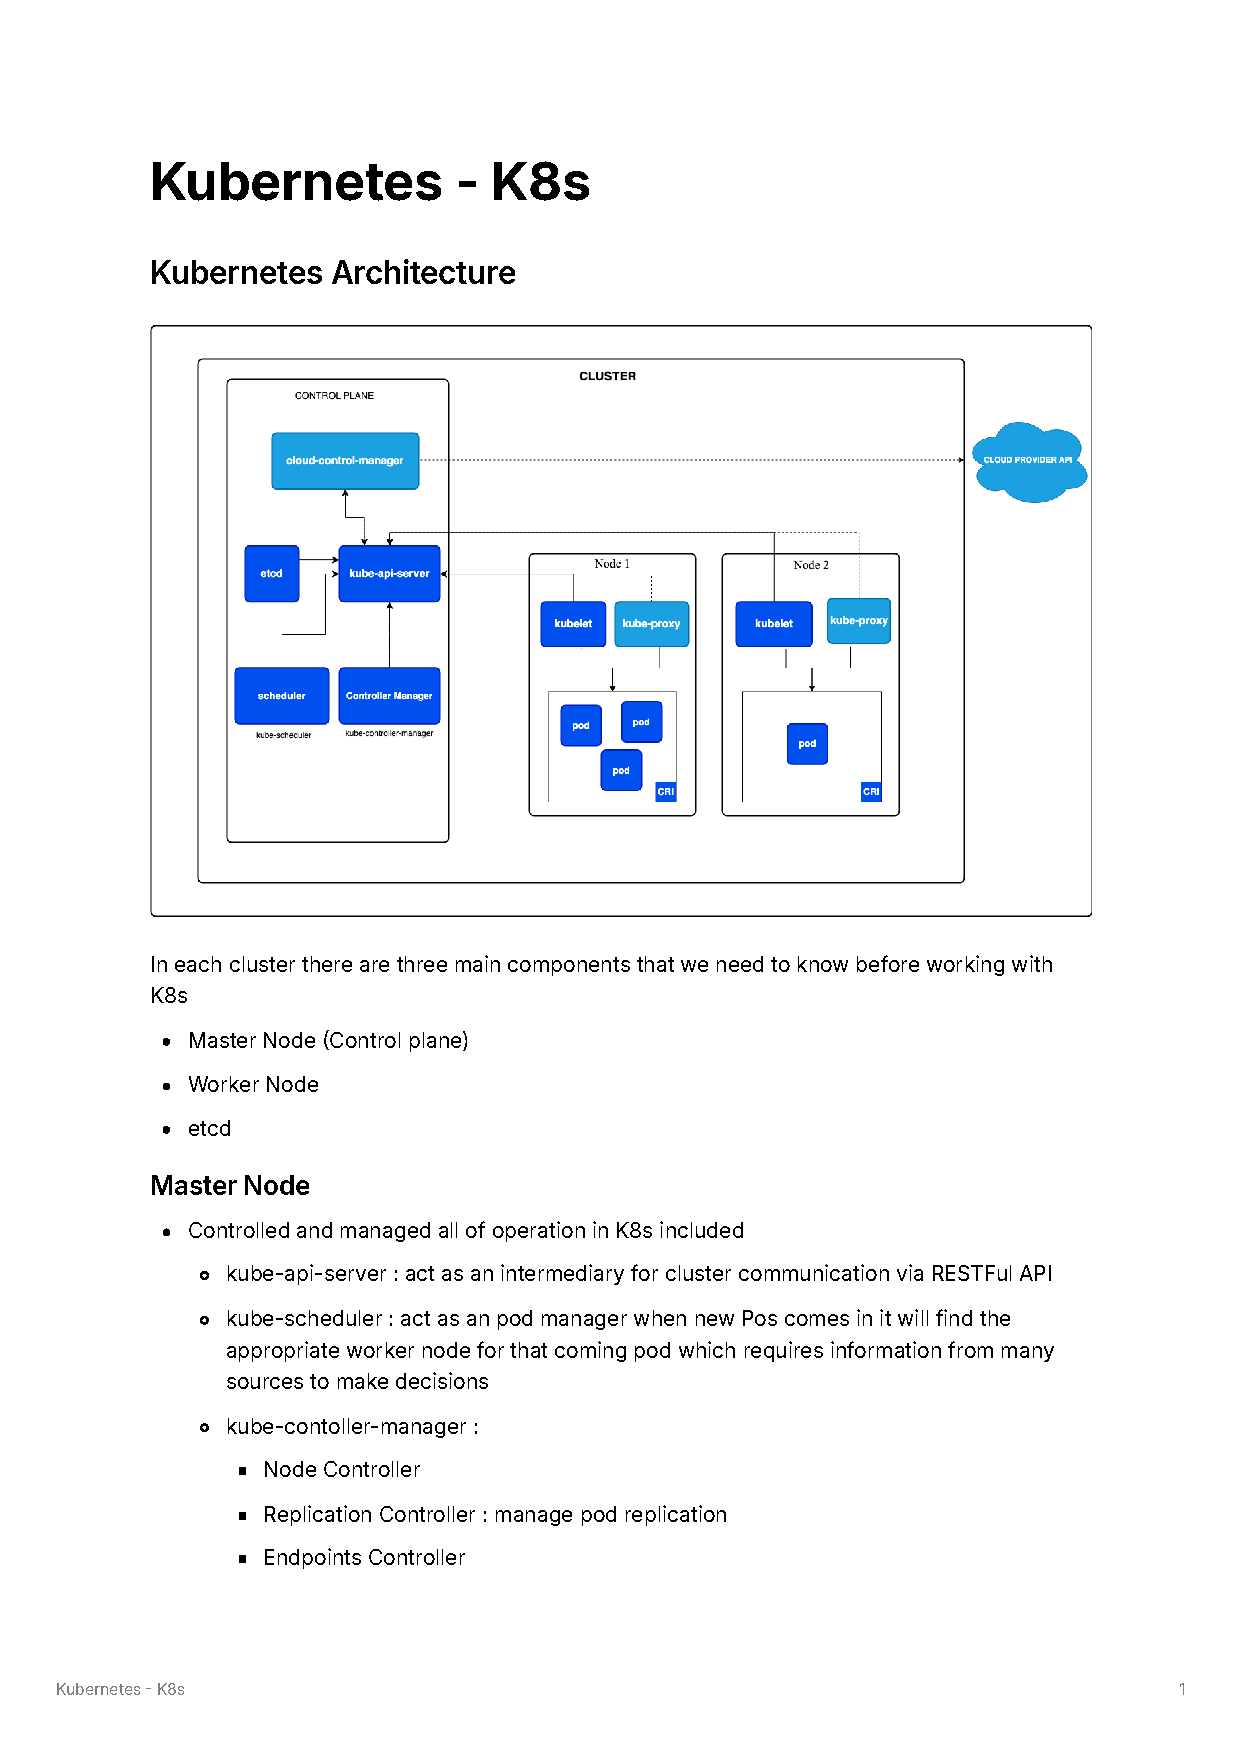
\includepdf[pages=-, scale=.8, pagecommand={\hypertarget{target:kube}{},\label{page:kube}}, nup=1x1, frame=true]{pdf/kube}
\includepdf[pages=-, scale=.8, pagecommand={\hypertarget{target:jenkins}{},\label{page:jenkins}}, nup=1x1, frame=true]{pdf/jenkins}
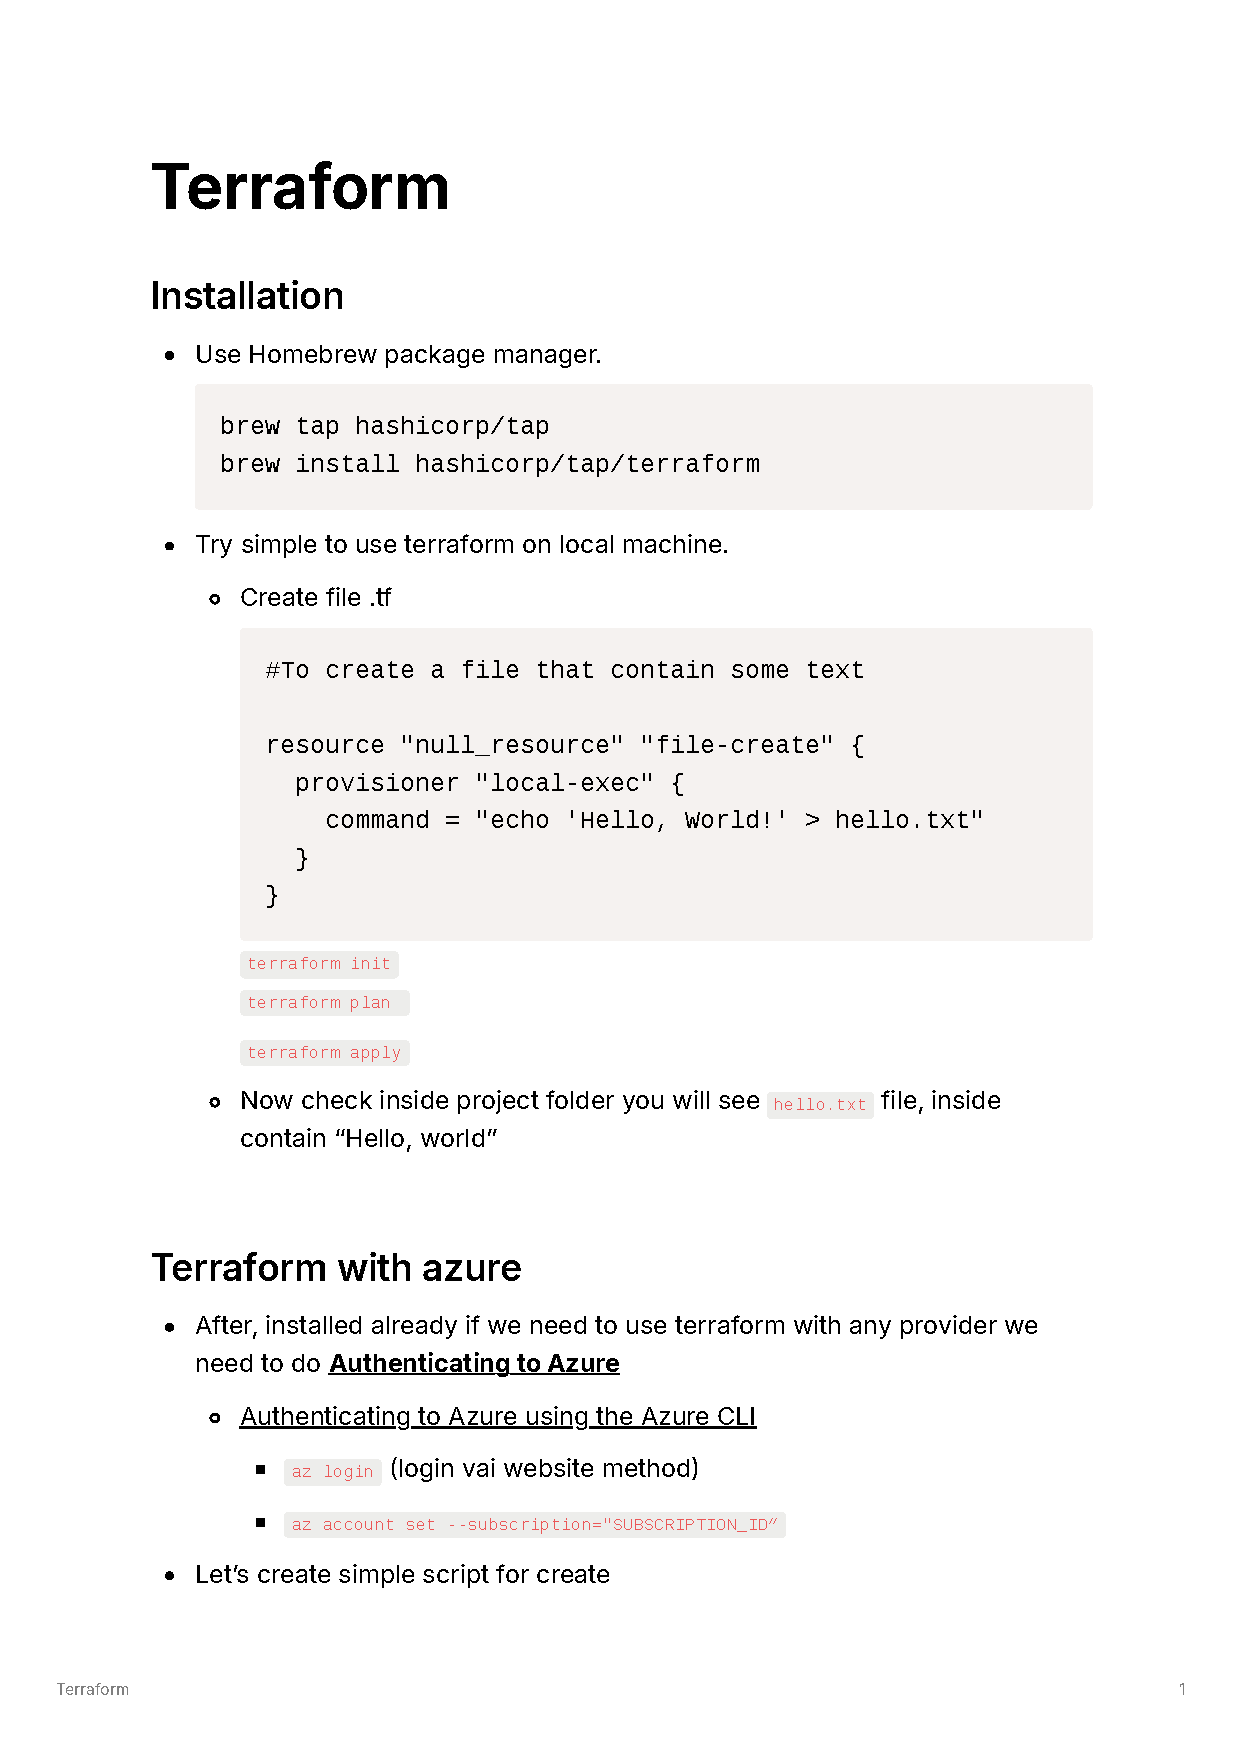
\includepdf[pages=-, scale=.8, pagecommand={\hypertarget{target:terraform}{},\label{page:terraform}}, nup=1x1, frame=true]{pdf/terraform}
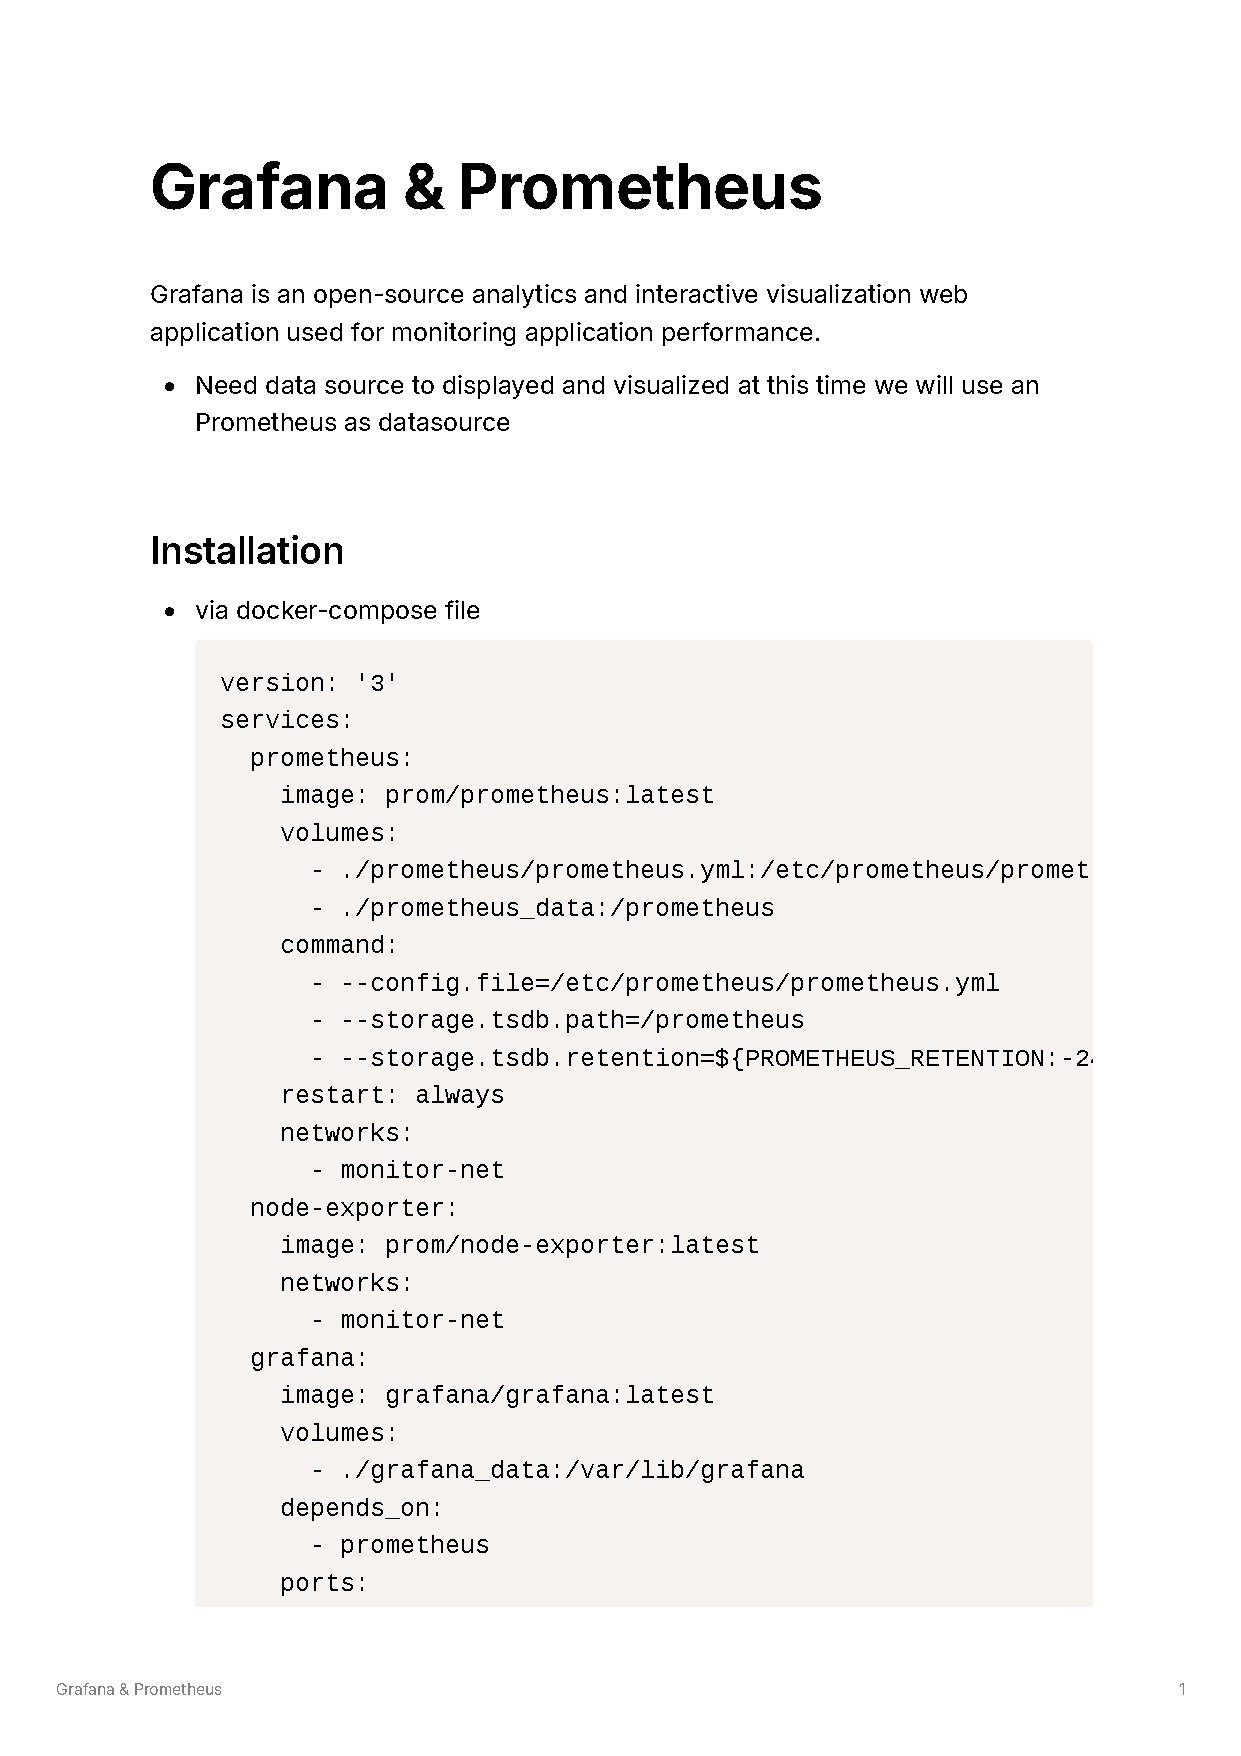
\includepdf[pages=-, scale=.8, pagecommand={\hypertarget{target:monitoring}{},\label{page:monitoring}}, nup=1x1, frame=true]{pdf/monitoring}
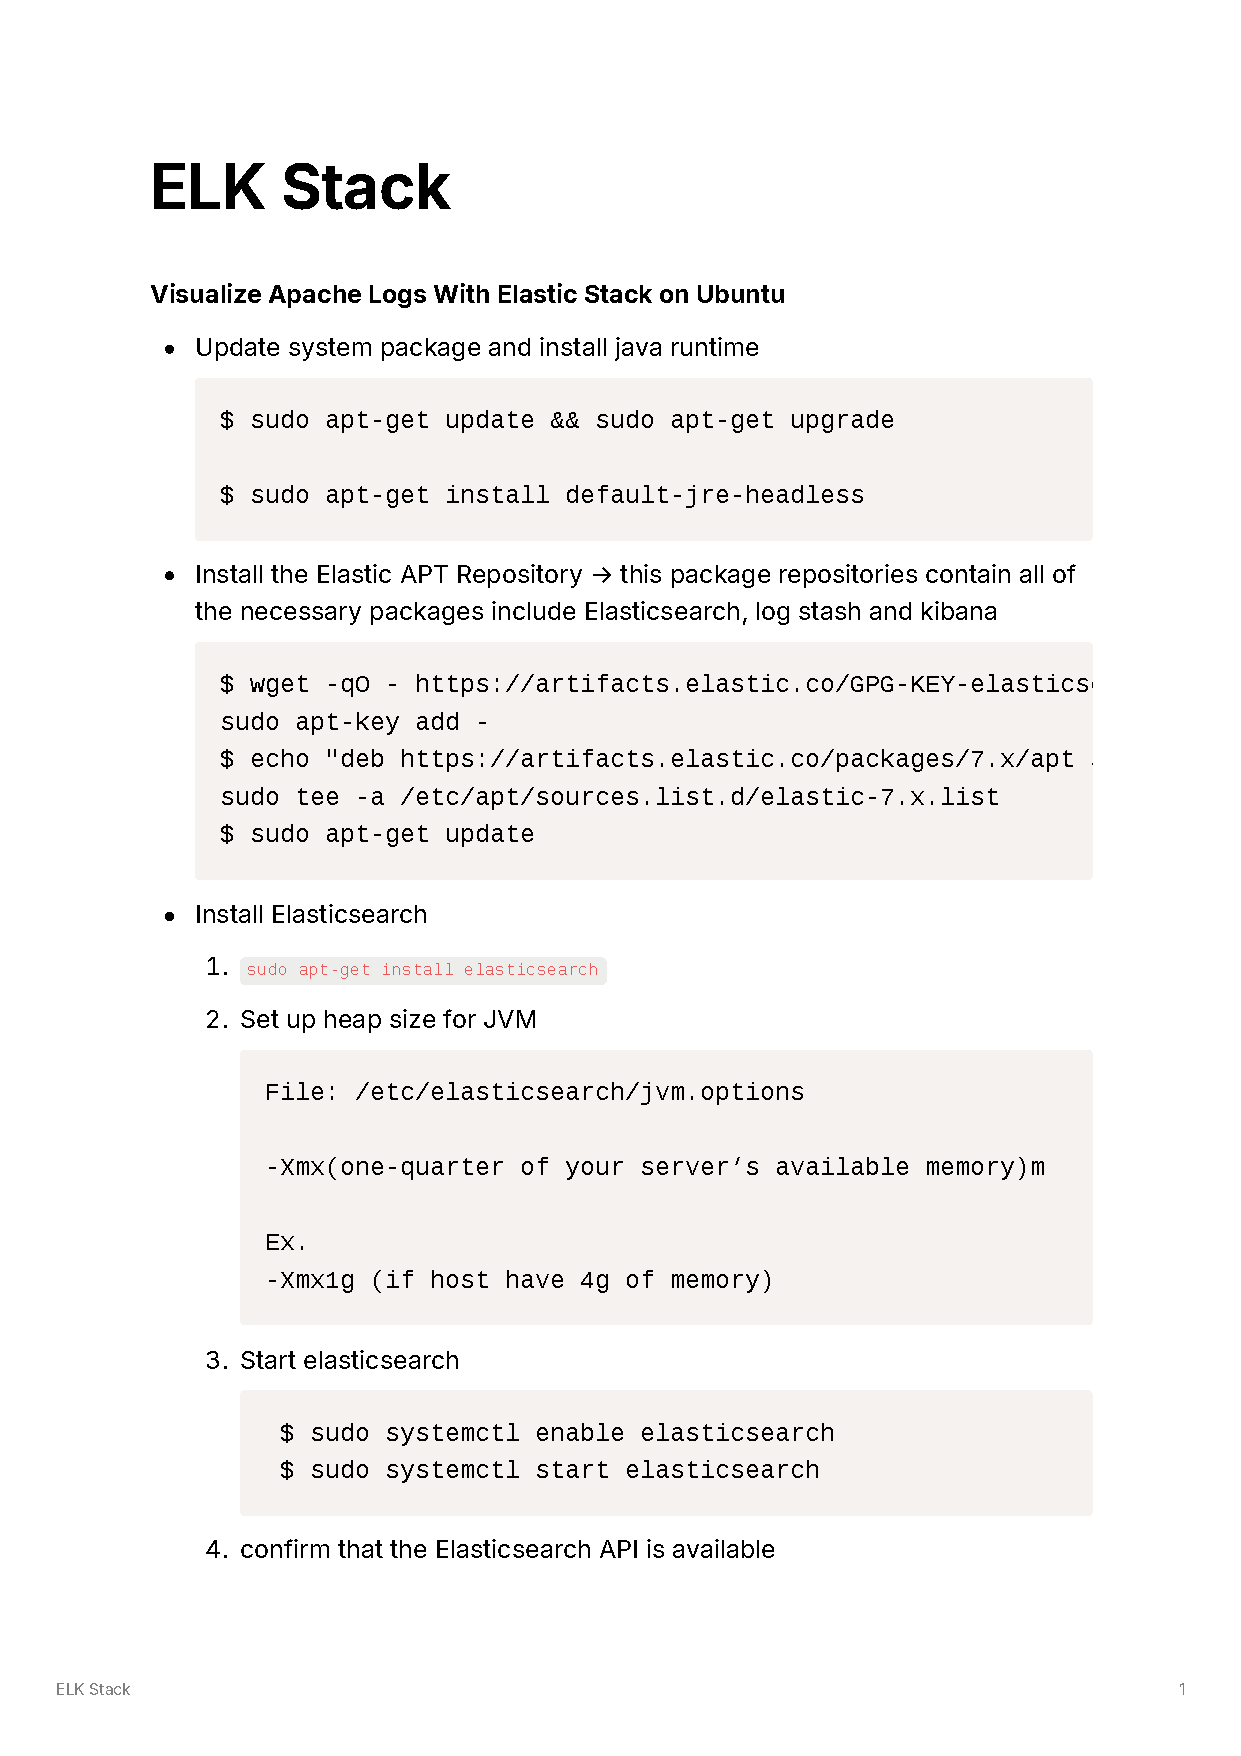
\includepdf[pages=-, scale=.8, pagecommand={\hypertarget{target:elk}{},\label{page:elk}}, nup=1x1, frame=true]{pdf/elk}

  %% Display glossary (optional) -- need glossary option.
  \ifglossary\glossarypage\fi

  %% Display index (optional) -- need idx option.
  \ifindex\indexpage\fi
\fi % \ifproject
\end{document}
